%%%%%%%%%%%%%%%%%%%%%%%%%%%%%%%%%%%%%%%%%%%%%%%%%%%%%%%%%%%%%%%%%%%%%%%%%%%%%%%%%%%%%%%%%%%%%%%%%%%%%%%%%%%%%%%%%%%%%%%%%%%%%%%%%%%%%%%%%%%%%%%%%%%%%%%%%%%
% This is just an example/guide for you to refer to when submitting manuscripts to Frontiers, it is not mandatory to use Frontiers .cls files nor frontiers.tex  %
% This will only generate the Manuscript, the final article will be typeset by Frontiers after acceptance.   
%                                              %
%                                                                                                                                                         %
% When submitting your files, remember to upload this *tex file, the pdf generated with it, the *bib file (if bibliography is not within the *tex) and all the figures.
%%%%%%%%%%%%%%%%%%%%%%%%%%%%%%%%%%%%%%%%%%%%%%%%%%%%%%%%%%%%%%%%%%%%%%%%%%%%%%%%%%%%%%%%%%%%%%%%%%%%%%%%%%%%%%%%%%%%%%%%%%%%%%%%%%%%%%%%%%%%%%%%%%%%%%%%%%%

%%% Version 3.4 Generated 2018/06/15 %%%
%%% You will need to have the following packages installed: datetime, fmtcount, etoolbox, fcprefix, which are normally inlcuded in WinEdt. %%%
%%% In http://www.ctan.org/ you can find the packages and how to install them, if necessary. %%%
%%%  NB logo1.jpg is required in the path in order to correctly compile front page header %%%

\documentclass[utf8]{frontiersSCNS} % for Science, Engineering and Humanities and Social Sciences articles
%\documentclass[utf8]{frontiersHLTH} % for Health articles
%\documentclass[utf8]{frontiersFPHY} % for Physics and Applied Mathematics and Statistics articles

%\setcitestyle{square} % for Physics and Applied Mathematics and Statistics articles
\usepackage{url,hyperref,lineno,microtype,subcaption}
\usepackage[onehalfspacing]{setspace}
\epstopdfsetup{outdir=./}

\linenumbers


% Leave a blank line between paragraphs instead of using \\


\def\keyFont{\fontsize{8}{11}\helveticabold }
\def\firstAuthorLast{Mrad {et~al.}} %use et al only if is more than 1 author
\def\Authors{Assaad Mrad\,$^{1,*}$, Sanna Sevanto\,$^{2}$, Jean-Christophe Domec\,$^{1,3}$, Yanlan Liu\,$^{1}$, Mazen Nakad\,$^{1}$ and Gabriel Katul\,$^{1,4}$}
% Affiliations should be keyed to the author's name with superscript numbers and be listed as follows: Laboratory, Institute, Department, Organization, City, State abbreviation (USA, Canada, Australia), and Country (without detailed address information such as city zip codes or street names).
% If one of the authors has a change of address, list the new address below the correspondence details using a superscript symbol and use the same symbol to indicate the author in the author list.
\def\Address{$^{1}$Nicholas School of the Environment, Duke University, Durham, NC, USA \\
$^{2}$Earth and Environmental Sciences Division, Los Alamos National Laboratory, Los Alamos, New Mexico, USA \\
$^{3}$ UMR INRA-ISPA 1391, Bordeaux Sciences Agro, Gradignan 33195, France \\
$^{4}$Department of Civil and Environmental Engineering, Duke University, Durham, NC}
% The Corresponding Author should be marked with an asterisk
% Provide the exact contact address (this time including street name and city zip code) and email of the corresponding author
\def\corrAuthor{Assaad Mrad}

\def\corrEmail{mradassaad2@gmail.com}




\begin{document}
\onecolumn
\firstpage{1}

\title[Dynamic optimality principle for water use strategies]{A dynamic optimality principle for water use strategies explains isohydric to anisohydric plant responses to drought} 

\author[\firstAuthorLast ]{\Authors} %This field will be automatically populated
\address{} %This field will be automatically populated
\correspondance{} %This field will be automatically populated

\extraAuth{}% If there are more than 1 corresponding author, comment this line and uncomment the next one.
%\extraAuth{corresponding Author2 \\ Laboratory X2, Institute X2, Department X2, Organization X2, Street X2, City X2 , State XX2 (only USA, Canada and Australia), Zip Code2, X2 Country X2, email2@uni2.edu}


\maketitle


\begin{abstract}

%%% Leave the Abstract empty if your article does not require one, please see the Summary Table for full details.


% As a primary goal, the abstract should render the general significance and conceptual advance of the work clearly accessible to a broad readership. References should not be cited in the abstract. Leave the Abstract empty if your article does not require one, please see \href{http://www.frontiersin.org/about/AuthorGuidelines#SummaryTable}{Summary Table} for details according to article type. 

Optimality principles that underlie models of stomatal kinetics require identifying and formulating the gain and the costs involved in opening stomata. While the gain has been linked to larger carbon acquisition, there is still debate as to the costs that limit stomatal opening. This work presents an Euler-Lagrange framework that accommodates water use strategy and various costs through the formulation of constraints. The reduction in plant hydraulic conductance due to cavitation is added as a new constraint above and beyond the hydrological balance and analyzed for three different types of whole-plant vulnerability curves. Model results show that differences in vulnerability curves alone lead to relatively iso- and aniso-hydric stomatal behavior. Moreover, this framework explains how the presence of competition (biotic or abiotic) for water alters stomatal response to declining soil water content. This contribution corroborates previous research that predicts that a plant's environment (e.g., competition, soil processes) significantly affects its response to drought and supplies the required mathematical machinery to represent this complexity. The method adopted here disentangles cause and effect of the opening and closure of stomata and complements recent mechanistic models of stomatal response to drought.


\tiny
 \keyFont{ \section{Keywords:} Drought, dynamic optimality, isohydricity and anisohydricity, photosynthesis,  plant hydraulics, stomata, transpiration, water use strategy, } %All article types: you may provide up to 8 keywords; at least 5 are mandatory.
\end{abstract}

\section{Introduction}

Some two centuries after the original experiments of Francis Darwin \citep{darwin1898ix,scarth1927stomatal}, the significance of stomatal kinetics in climate, atmospheric, hydrologic, agricultural, and ecosystem sciences is not in dispute \citep{hetherington2003role}.  The exchange of water vapor and CO$_2$ between the atmosphere and plants is regulated by a dynamic stomatal aperture. This impacts a plethora of processes such as CO$_2$ concentration in the atmosphere ($c_a$) and positive feedbacks on air temperature \citep{cox2000acceleration} as well as water cycling \citep{betts2007projected,katul2012evapotranspiration}, sensible heat flux, and boundary layer dynamics regulating predisposition of rainfall \citep{siqueira2009soil, manoli2016soil}. Other impacted processes also include pollutant uptake such as tropospheric ozone and concomitant plant damage \citep{rich1964ozone,musselman2006critical}, antecedent soil moisture content and flash-flooding \citep{javelle2010flash}, silviculture and forest management \citep{makela1986stand}, irrigation water requirements and profitable crop yield estimation \citep{vico2015ecohydrology} to name a few.  What remains the subject of inquiry is how to represent stomatal kinetics for the above applications parsimoniously. 

Numerous models for stomatal kinetics have emerged over the past century or so (for an overview see e.g. \citet{jarvis1976interpretation,collatz_physiological_1991,leuning_critical_1995,damour2010overview,way2011well} ). These studies rely on two points.  The first is that stomatal kinetics cannot be considered in isolation as they are impacted by exogenous environmental variables \citep{jarvis1976interpretation,pearcy1990sunflecks,mott1991stomatal,medlyn_temperature_2002} such as photosynthetically active radiation (PAR), air temperature ($T_a$), vapor pressure deficit (VPD), and $c_a$. This is in addition to the effects of endogenous variables impacted by soil-root-plant processes such as soil, rhizosphere and plant hydraulics \citep{sperry_hydraulic_2000, brodribb_relations_2003}, osmoregulation and carbohydrate export from the leaf \citep{nikinmaa_assimilate_2013,sevanto_how_2014,jensen2016sap,konrad2018xylem} to name a few. The second point is that optimization approaches based on maximum fitness offer a whole-system framework to begin tackling the description of stomatal kinetics \citep{manzoni_optimizing_2011,manzoni_optimization_2013,huang2018transport}. Because photosynthesis is the main source of carbon used by plants for numerous functions such as growth and defenses \citep{novick2012increased}, maximizing fitness is akin to maximizing photosynthesis over a preset time scale yet to be determined \citep{cowan1971relative,givnish1976sizes,cowan_stomatal_1977,dewar2010maximum}.  This approach is appealing because the mathematical framework to be employed (i.e., variational principles) has been used in numerous branches of science \citep{witelski_variational_2015}.  The barriers of this approach are not in the formulation of the 'functional' to be maximized (i.e., photosynthesis) but in the constraints and costs to be imposed on such an optimization \citep{dewar2018new}.  Naturally, these constraints and costs operate over time scales that may be difficult to determine a \textit{priori}.  Early work relying on variational principles focused on maximizing photosynthesis by setting costs (in carbon units) as transpirational losses from leaves  \citep{cowan_stomatal_1977,cowan_stomatal_1978}. 
Other versions of this approach maximize instantaneous carbon gain for a given finite amount of water loss per unit leaf area \citep{katul_leaf_2009}.  A recent approach seeks instantaneous maximization of gains and assumes that plant hydraulics control stomatal opening trends.  The approach is now labelled as a profit-maximization model for stomatal kinetics \citep{sperry_pragmatic_2016,sperry_predicting_2017}. The profit-maximization scheme formulates the cost based on a relative loss in plant hydraulic conductance.  Other optimization variants have also been proposed based on maintaining constant inter-cellular to ambient atmospheric CO$_2$ concentration ratio \citep{prentice2014balancing} or maximizing carbon transport out of the leaves through the phloem \citep{nikinmaa_assimilate_2013}.  In the constant internal-to-ambient CO$_2$ concentration ratio approach, the objective is to minimize instantaneous cost (instead of maximizing gains) of maintaining the transpirational stream required to support photosynthesis while maintaining photosynthetic proteins at levels required to support assimilation rates.  Predictions from all these approaches have received experimental support under wide-ranging conditions despite differences in formulating costs  \citep{nikinmaa_assimilate_2013,prentice2014balancing,sperry_predicting_2017}.
The past five decades have witnessed a renaissance in the development and use of optimization theories to describe stomatal kinetics. This renaissance led to the revision of the nature of the costs associated with photosynthetic gains to include soil-plant hydraulics, soil water availability, energy limitations \citep{roth2018fossil} among others, and are all gaining prominence and partial experimental support. What is missing is a general framework that can (i) recover the various optimization schemes already proposed and (ii) explicitly link these schemes with plant water use strategies (WUS). This work interprets WUS as the relative importance prescribed to instantaneous versus delayed gains. A conservative plant is one that prescribes more importance to delayed gains than a relatively aggressive one. This interpretation was first introduced mathematically elsewhere \citep{manzoni_optimization_2013} and is built upon in the current article.

The work here aims to establish the blueprint of a calculus of variations based framework using plant hydraulics and droughts as case studies.  The focus on droughts is purposeful because of the recent interest in plant-water use strategies during droughts, and ways of defining and measuring isohydricity \citep{franks_anisohydric_2007,martinezvilalta_new_2014,meinzer_mapping_2016}.  Such analysis requires a re-formulation of the conventional optimization problem to satisfy all constraints at a sub-daily time scale while maximizing carbon gain over a dry-down period. A dry-down period is here defined as the period of time in between consecutive rainfall events. The multiplicity of time scales exists to both explicitly accommodate variable environmental drivers and abiotic (e.g., drainage) as well as biotic (i.e., overlapping rooting zones of adjacent plants) competition for water and optimize plant fitness (here seen as total carbon assimilated). The theoretical framework to be employed is based on the calculus of variations and dynamic optimization principles because they allow for (i) directly accounting for plant-water use strategies (i.e. aggressive versus conservative water users), (ii) using multiple constraints (hydrologic balance, energy balance, etc...), and  (iii) extending the deterministic analysis used here to a stochastic framework (at least for rainfall) using conventional approaches  \citep{cowan1986economics,makela1996optimal,manzoni_optimization_2013,lu2016optimal}.  Setting a 'carbon value' to the terminal soil moisture content around the rooting zone at the end of the dry-down period allows mathematically assigning a plant water use strategy \citep{manzoni_optimization_2013}.   The focus of the work here will be restricted to the aforementioned point (i) so as to demonstrate the utility of the proposed approach here and leave points (ii) and (iii) for future inquiry and extensions of the proposed method. It is not the goal of the current article to complexify the computational needs so as to achieve good agreement with a particular site or study. The main contribution here is the presentation of the mathematical machinery required to add hydraulic (and other) limitations to the traditional and widely used optimization principle for stomatal behavior \citep{cowan_stomatal_1977,cowan1986economics}. The optimization scheme developed by Cowan and others in 1977 has been shown to perform well with data in the past \citep{dubois_2007,gu_2010}. The rest of the document will discuss what amendments are needed to extend this framework to drought studies.  The approach will be compared with a controlled experiment \citep{venturas_2018} that was used to test the profit maximization scheme.

As a guide to the development of this framework, the work answers the following question: To what degree does water use strategy dictate stomatal control during dry-down? In a recent review of the theory of optimal stomatal control, \citet{buckley_optimal_2017} emphasized the importance of delayed benefits such as keeping soil moisture at higher levels for future use, which is accommodated here using a terminal gain. The optimization scheme proposed explores the consequences of WUS and choices made about soil-plant hydraulic strategy, and whether few but important plant hydraulic traits alone are capable of mapping stomatal behavior anywhere on the iso-anisohydric spectrum. In particular, the model behavior is discussed in the water demand and supply limited cases to demonstrate the influence of competition on plant water use for trees of three different hydraulic vulnerability (to embolism)  curves (VCs). Another point of departure from previous analyses based on treating $g_s$ as the control variable is that soil-plant hydraulics limit plant transpiration when atmospheric water demand exceeds the supply of water provided by the soil and xylem. This limitation imposes an upper bound on $g_s$. The newly proposed model results are then compared with recent profit maximization approach. 

\section{Materials and Methods}

This section will first present a review of the calculus of variation applied to plant photosythensis and then describe an alteration to mathematically formalize the concept of Water Use Strategy (WUS). The WUS concept recognizes that for the same plant hydraulic, allometric, and photosynthetic traits, a plant can adopt a spectrum of water use intensities varying from aggressive to conservative. The third sub-section relates carbon fixation to $g_s$ and details the assumptions adopted. The fourth and fifth sub-sections develop conservation of water mass equations needed to obtain physically plausible results. The third and fifth sub-sections combined are the analytical basis of the carbon gain and water loss trade-off with stomatal opening. The sixth sub-section explains the mathematical machinery behind maximizing carbon gain while combining the objectives, formulations, and constraints developed in the previous sub-sections. The seventh sub-section details the gain-risk model used for comparison \citep{sperry_what_2015,sperry_pragmatic_2016}. The eighth and final sub-section explains the values of parameters used, which species was modeled, and the test cases chosen to run the model.

\subsection{Theory: calculus of variations}

The principle adopted here is that plants maximize their carbon gain ($A$) over a dry-down period $T$ selected to be the mean inter-storm period. This principle assumes that plants control $g_s$ per unit leaf area under constraints. Previous work constrained control of $g_s$ by enforcing the daily water balance at the soil level \citep{manzoni_optimization_2013}. To mathematically express this principle under the mentioned constraint, an augmented Lagrangian is defined $L$:
\begin{equation}
    \label{eqn:Lagrangian}
    L\Big(g_s, x, \frac{dx}{dt}, \lambda, t\Big) = A(g_s, t) - \lambda \Bigg[ \frac{dx}{dt} - f_e\Big(g_s, x, \frac{dx}{dt}, t\Big)\Bigg],
\end{equation}
where $\lambda$ is the Lagrange multiplier in mol mol$^{-1}$ known as the instantaneous marginal water use efficiency in ecological terms; $x$ is the relative soil moisture content or degree of saturation in the rooting zone bounded between zero (dry soil) and unity (all pores are filled with water); $t$ is time in days; and $f_e$ is the summation of all soil hydrological fluxes in days$^{-1}$.

Because the approach states that $A$ is maximized over a period $T$ rather than instantaneously, the objective function $J$ integrates $L$ from $t=0$ signifying the beginning of a dry down to $t=T$ at the end of it:
\begin{equation}
    \label{eqn:Objective}
    J\Big(g_s, x, \frac{dx}{dt}, \lambda, t\Big) = \int_0^T L\Big(g_s, x, \frac{dx}{dt}, \lambda, t\Big).
\end{equation}
The goal then consists of finding the function $g_s(t)$ in terms of $t$ that maximizes $J$ over the period $T$. This goal is achieved by solving the Euler-Lagrange equations using the calculus of variations \citep{witelski_variational_2015}. This approach requires expressing $A$ and $f_e$ as functions of the control variable $g_s$ and the state variable $x$, which are now discussed. Again, while $L$ is maximized over a drydown period $T$, $g_s$, $x$, its derivative, and $\lambda$ are all resolved at sub-daily or diurnal time scale.

\subsection{Water use strategy (WUS)}

A terminal gain term is added to $J$ to include the effects of water use strategy (WUS) \citep{manzoni_optimization_2013}. The revised objective function $J$ is now:
\begin{equation}
    \label{eqn:Objective_WUS}
    J_{\text{WUS}} = \int_0^{T} L\Big(g_s, x, \frac{dx}{dt},\lambda,t \Big) dt + J_{T},
\end{equation}
where $J_T$ is the terminal gain term. $J_T$ may take multiple forms but should represent the costs of aggressively opening stomata regardless of drought. For simplicity, $J_T$ may be interpreted as the carbon value of the terminal soil water moisture $x(T)$ prescribed as:
\begin{equation}
    \label{eqn:terminal_gain}
    J_{T} = \Lambda x(T),
\end{equation}
where the introduced parameter $\Lambda$ in mol mol$^{-1}$ sets the carbon value of $x(T)$. Larger $\Lambda$ represents a more conservative WUS and vice versa \citep{manzoni_optimization_2013}. Ecologically, the terminal gain $J_{T}$ as expressed in equation \ref{eqn:terminal_gain} prevents excessive and detrimental use of water especially during a short dry-down period (i.e., small $T$). As will be shown in the 'Maximizing the objective' sub-section below, the value of $J_T$, as expressed in equation \ref{eqn:terminal_gain}, can be inferred experimentally in water stressed environments by observing the marginal water use efficiency ($\lambda$) of a plant under dry soil. 

The plant could now 'maximize' its objective $J_{\text{WUS}}$ by keeping a high $x(T)$ at the end of dry-down. A higher $x(T)$ means higher potential carbon gains after drought, limited loss in root to leaf hydraulic conductance, among other advantages.  The magnitude of $J_{T}$ should be interpreted with consideration of the length of the dry-down period ($T$). The same $J_{T}$ contributes to a smaller portion of the objective function for a longer dry-down period (Equation \ref{eqn:terminal_gain}). In this study, the length of the dry-down period is fixed across all experiments as it is presumed to be externally imposed on the soil-plant system by the precipitation regime. Future studies will assume this quantity randomly distributed set by the actual instead of the mean inter-storm period.  Throughout, $J_{\text{WUS}}$ will be the objective to be maximized instead of $J$ of equation \ref{eqn:Objective}.

\subsection{Carbon gain}

The biochemical demand ($A_{demand}$) for atmospheric CO$_2$ for a C3 leaf is either limited by the Ribulose-1,5-bisphosphate carboxylase/oxygenase (Rubisco) enzyme activity under saturated incoming PAR or by Ribulose-1,5-biphosphate (RuBP) activity under limiting incoming PAR \citep{farquhar_biochemical_1980}. To consider both limitations using a differentiable function that facilitates numerical optimization, $A_{demand}$ is calculated using the co-limitation approach as \citep{vico_perspective_2013}:
\begin{equation}
    \label{eqn:vico_model}
    A_{demand} = k_1 \frac{c_i - \Gamma^*}{c_i + k_2},
\end{equation}
where $c_i$ is the carbon dioxide concentration in the intercellular spaces of the leaf assumed to be equal to the concentration inside the chloroplast (infinite mesophyll conductance); $\Gamma^*$ is the CO$_2$ compensation point defined by the $c_i$ where carbon dioxide assimilation rate ceases and also a function of leaf temperature; $k_1$ and $k_2$ are parameters determined from Rubisco and RuBP limits as described elsewhere \citep{vico_perspective_2013}. Namely, $k_1 = \frac{j}{4}$ where $j$ is the electron transport rate and $k_2 = \frac{j}{4} \frac{a_2}{V_{c,max}}$ where $V_{c,max}$ is the maximum carboxylation rate. The $a_2 = K_c (1+O_a/K_o)$ where $K_c$ and $K_o$ are Michaelis-Menten constants for CO$_2$ and O$_2$ respectively and $O_a$ is the atmospheric concentration of oxygen \citep{bernacchi_improved_2001}. The inclusion of a mesophyll conductance is possible but is left for future work because of the empirical nature of its formulation \citep{dewar2018new}.

% Throughout, it is assumed that the boundary layer conductance surrounding each leaf is negligible such that the leaf temperature is the same as $T_a$.
% I think this should be said somewhere that glb is not accounted for because we assume it to be very large (>100 times gs)

The parameters of equation \ref{eqn:vico_model} ($V_{c,max}$, $\Gamma^*$, $K_c$, $K_o$) are leaf temperature dependent while $j$ is both leaf temperature and PAR dependent \citep{medlyn_temperature_2002}. The formulations describing the dependence of $K_c$, $K_o$, and $\Gamma^*$ on leaf temperature are conventional and are described elsewhere \citep{bernacchi_improved_2001}. The $j_{max}$ and $V_{c,max}$ dependencies on temperature are taken from prior studies for \textit{Pinus pinaster} \citep{medlyn_temperature_2002} while the optimal values $j_{opt}$ and $V_{c,opt}$ were selected to match those of \textit{Pinus ponderosa} at a reference temperature of 25$^o$C, the dominant species in the ecosystem used as a case study (see subsection Environmental data and plant species and property selection).

For simplicity, the approximations used for $A_{demand}$ in equation \ref{eqn:vico_model} neglect 1) the potential limitation by sucrose synthesis, 2) the contribution by dark respiration to $A_{demand}$, and 3) the temperature buffering effect of the leaf boundary layer such that leaf temperature equals atmospheric temperature $T_a$ (boundary layer conductance assumed very high compared to $g_s$).  The latter approximation avoids the need for specifying wind speed variations and turbulent intensity within the canopy.  The inclusion of a leaf energy balance to accommodate the difference between air and surface temperature is possible by formulating another constraint beyond the hydrologic balance here \citep{roth2018fossil} but this extension will not be elaborated upon here.  It was shown elsewhere that such an addition introduces another Lagrange multiplier (arising from the energy balance constraints) that can be lumped with the original Lagrange multiplier without altering the character of the Euler-Lagrange equation \citep{roth2018fossil}.

When every CO$_2$ molecule captured from the atmosphere by the leaf is assimilated, $A_{demand} = A_{supply}$. A Fickian diffusion represents the supply of carbon dioxide from the atmosphere into the intercellular space with a diffusivity that depends on stomatal kinetics:
\begin{equation}
    \label{eqn:supply}
    A_{supply} = g_s (c_a - c_i),
\end{equation}
where $c_a$ is, as before, the atmospheric concentration of CO$_2$ in mol mol$^{-1}$.
% To determine the carbon dioxide concentration inside the chloroplast, we adopt a relation developed elsewhere \citep{dewar2018new}:
% \begin{equation}
%     \label{eqn:dewar_mes}
%     c_c - \Gamma^* = \varphi(c_i - \Gamma^*)
% \end{equation}
% where $\varphi = 1 - \frac{\psi_l}{\psi_c}$ is used as a reduction factor and $\psi_c$ is the critical leaf water potential whose numerical value is defined below and $\psi_l$ is the actual leaf water potential. 

Combining equations \ref{eqn:vico_model} and \ref{eqn:supply}, a formulation for $A$ in terms of $g_s$ that is explicitly independent from $c_i$ is obtained and given as:
\begin{equation}
    \label{eqn:A_noci}
    A = \frac{1}{2} [g_s (c_a + k_2) + k_1 - \sigma],
\end{equation}
where $\sigma = \sqrt{-4 g_s k_1(c_a - \Gamma^*) + (c_a g_s + k_2 g_s + k_1)^2} $.  Because $\sigma$ is positive and monotonically increasing with $g_s$, the $A$-$g_s$ relation is a concave function, a necessary condition for optimal behavior as discussed elsewhere \citep{katul_stomatal_2009}. To sum up, when the temporal variations in $T_a$ and PAR are specified along with $c_a$ and $O_a$, the $g_s$ is the only independent variable in equation \ref{eqn:A_noci}.

\subsection{Soil water balance}
% The ensure the continuity of the water stream throughout the tree, we model three vertically connected layers: the soil, the trunk and branches, and the leaves. Each of these layers are characterized by a hydraulic resistance that is non-linearly related to water potential. Prescribing hydraulic resistances to these different layers allows computation of quantities regarded as indicative of isohydric to anisohydric behaviour. Such quantities include leaf water potential ($\psi_l$) and stomatal conductance ($g_s$).

Plant water use is bound by conservation of mass at every point along the soil, plant, atmosphere continuum. This and the following sub-section formulate water balance at the soil and leaf level to ensure correct accounting of water mass. The resulting equations will set physical boundaries on the optimization scheme described above.

During a dry-down, soil-water balance must be satisfied at every instant $(t \in [0,T])$. In the absence of precipitation, the soil-water balance can be expressed as \citep{rodriguez-iturbe_ecohydrology_2007}:
\begin{equation}
    \label{eqn:soil_water}
    \frac{dx(t)}{dt} = f_e\Big(g_s, x, \frac{dx}{dt}, t\Big) = \frac{\nu}{ n Z_r}[- E(g_s, t) - U(x, t)],
\end{equation}
where $U$ lumps all the uncontrolled losses (independent of the plant) in mmol m$^{-2}$ s$^{-1}$. These may account for soil water leakage away from the rooting zone, evaporation from the soil surface, and competition from other plant roots; E is the transpiration rate from the plant in mmol m$^{-2}$ s$^{-1}$ (throughout, water fluxes are expressed per unit leaf area);  $n$ is the soil porosity in m$^3$ m$^{-3}$; and $Z_r$ is the effective plant rooting depth in $m$. To ensure dimensional equivalence, the right hand side is multiplied by $\nu = \text{LAI} \, M_w \times 24 \times 3600 / \rho_w$, LAI is the leaf area index in m$^3$ m$^{-3}$, $M_w = 18 \times 10^{-6}$ kg mmol$^{-1}$ is the molar weight of water, and $\rho_w = 1000$ kg m$^{-3}$ is its density. Therefore, the factor on the right hand side of equation \ref{eqn:soil_water} converts the fluxes $E$ and $U$ from molar fluxes to volumetric fluxes, converts their rate from s$^{-1}$ to days${^{-1}}$, and normalizes these fluxes by the effective rooting depth.

As part of $U$, soil leakage is modeled as gravitational drainage such that water losses from leakage per unit soil area and unit depth are determined by the soil hydraulic conductivity $g_x$ \citep{campbell_introduction_2012}:
\begin{equation}
    \label{eqn:soil_cond}
    g_x = g_{x,sat}x^{2b+3},
\end{equation}
where $g_{x,sat}$ is the soil conductivity near saturation and $b$ is a parameter determined from the soil water retention curve. Both parameters depend on pore structure that is linked to soil type using standard equations \citep{clapp_empirical_1978}. The soil water potential ($\psi_x$) can also be derived from the aforementioned soil water retention curve using:
\begin{equation}
    \label{eqn:Clapp_pot}
    \psi_x = \psi_{x,sat}x^{-b},
\end{equation}
where $\psi_{x,sat}$ is the soil water potential near field capacity.

The soil to root conductance $g_{sr}$ is assumed to be the conductivity of the soil $g_x$ divided by the distance between soil and root $l_{sr}$ estimated as $l_{sr} = \sqrt{d_r Z_r \text{RAI}}$ where $d_r$ is the fine root diameter in m and RAI is the root area index \citep{manzoni_optimization_2013}. If $g_x$ is given in kg s m$^{-3}$, then
\begin{equation}
    \label{eqn:soil_root}
    g_{sr} = \frac{10^3}{M_w \, \rho_w \, l_{sr} \, \text{LAI}} g_x, 
\end{equation}
where $g_{sr}$ now has units of mmol m$^{-2}$ MPa$^{-1}$ s$^{-1}$ and is expressed per unit leaf area for compatibility with the leaf-level water balance. Because the soil to root distance is taken into account in $g_{sr}$, one only needs to multiply $g_{sr}$ by the water potential difference between root and soil to obtain the flux of water from the soil into the roots. All the soil-root hydraulic properties are kept constant over the drydown period $T$ as shown in table \ref{tab:props}.

\subsection{Leaf-level water balance}

As a point of departure from previous analyses based on carbon gain maximization principles where the control variable is $g_s$, it is recognized that plant transpiration must be limited by soil-plant hydraulics when atmospheric water demand exceeds the potential supply of water from the soil pores. This limitation imposes an upper bound on $g_s$. 

An effective vulnerability describes the loss of conductivity of the whole plant system with decreasing water potential to embolism curve (VC). For simplicity, the VC of the entire hydraulic pathway (roots, trunk, branches, and leaves) is prescribed with a generic Weibull exceedance function \citep{sperry_what_2015}:
\begin{equation}
    \label{eqn:root_leaf}
    g_{rl} = g_{rl,max}exp\Big[-\Big(\frac{\psi}{\psi_{63}}\Big)^s\Big],
\end{equation}
where $g_{rl}$ is the root to leaf hydraulic conductance in mmol m$^{-2}$ MPa$^{-1}$ s$^{-1}$ expressed per unit leaf area, and $g_{rl,max}$ is its maximum value at saturation. The $\psi_{63}$ is the water potential at which the plant loses about 63\% of its conductance, as common in Weibull VCs. Finally, $s$ dictates the shape and curvature of the Weibull function. 
The $E$ at the soil, plant, and leaf levels must satisfy the continuity equation at steady-state:
\begin{equation}
    \label{eqn: mass_cons}
        \begin{split}
        E & = E_{demand} = 1.6\: g_s\, \text{VPD} \\
        & = E_{sr} = g_{sr}(\psi_x)(\psi_x - \psi_r)\\
        & = E_{rl} = \int_{\psi_l}^{\psi_r} g_{rl}(\psi) d\psi. \\
        \end{split}
\end{equation}
Here, $E_{demand}$ is the atmospheric demand of water, $E_{sr}$ is the soil to root water supply, $E_{rl}$ is the root to leaf supply. All expressions of $E$ are given in units of mmol m$^{-2}$ s$^{-1}$ expressed per unit leaf area. The $E_{rl}$ expression is analogous to porous media methods where it is recognized that water potential is not distributed hydrostatically along the medium.

It is noted that as $g_s$ varies with time, $\psi_l$ also varies in time to match supply and demand. The hydraulic constraint from the plant water supply system is apparent when one realizes that while $E_{demand}$ undergoes a limitless increase with rising $g_s$, water supply through $E_{sr}$ and $E_{rl}$ have maxima that cannot be exceeded due to concomitant decreases in hydraulic conductance functions $g_{sr}$ and $g_{rl}$ with increasing $\psi_x$, $\psi_r$, and $\psi_l$ (equations \ref{eqn:soil_root}, \ref{eqn:root_leaf}, and \ref{eqn: mass_cons}). The presence of a maximum possible water supply imposes an additional constraint on the stomatal conductance $g_s$.  

The $E_{rl}$ expression in equation \ref{eqn: mass_cons} only asymptotically reaches a maximum. So, for computational reasons, a critical transpiration rate $E_{crit}$ is now introduced to define a maximum possible water supply. The $E_{crit}$ is defined at the $\psi_l$ where the in series combination of soil-root $g_{sr}$ and root-leaf conductance is 5\% of its maximum values \citep{sperry_predicting_2017}. One finds this combined conductance by computing the partial derivative of $E$ with respect to $\psi_l$ such that the condition at $E$ becomes (see Appendix 1 for detailed derivations):
\begin{equation}
    \label{eqn:critical_E}
    \frac{\partial E}{\partial \psi_l} (\psi_l) = 0.05 \frac{\partial E}{\partial \psi_l} (\psi_x),
\end{equation}
where it is recognized that the maximum conductance of the whole water pathway at a certain $x$ will occur when all water potential are in equilibrium with $\psi_x$ due to the monotonically increasing nature of $g_{sr}$ and $g_{rl}$ (equations \ref{eqn:soil_root}, \ref{eqn:root_leaf}). At this condition, the critical leaf water potential $\psi_{l,crit}$ is attained as well as the corresponding critical root water potential $\psi_{r,crit}$ all being in equilibrium at $E = E_{crit}$.

This constraint of maximum transpiration rate can be imposed in the framework here using an additional Lagrange multiplier. Although mathematically neater, such a practice will lead to $\lambda$ in equation \ref{eqn:Lagrangian} losing its traditional definition of marginal water use efficiency. The maximum transpiration rate constraint is imposed in the following manner here so as to preserve this ecological interpretation of $\lambda$.  If maximizing $J_{\text{WUS}}$ (equation \ref{eqn:Objective_WUS}) leads to a $g_s$ that exceeds the maximum achievable $E$ ($E_{crit}$) at current $x$, this $g_s$ is replaced by its value when $E = E_{crit}$ to ensure that equation \ref{eqn:critical_E} is satisfied. Here, the assumption that plants take full advantage of their maximum transpiration capacity only applies to those intervals when $E$ exceeds $E_{crit}$ and is therefore forcibly set to its value at current $x$.

\subsection{Maximizing the objective}

From the definition of $J_{\text{WUS}}$ (equation \ref{eqn:Objective_WUS}), there are 5 independent variables: $g_s$, $x$, $dx / dt$, $\lambda$, and $t$. To maximize $J_{\text{WUS}}$, the calculus of variations \citep{witelski_variational_2015} is used to derive what are known as the Euler-Lagrange equations (see equation 3.55 in the mentioned reference). For this problem, these are a set of three equations to be simultaneously solved with two boundary conditions set on $x$ at the beginning of drydown ($x(0)$ at $t=0$) and on $\lambda$ at the end of the drydown period ($\lambda(T)$ at $t=T$). Solving these equations will yield the trends of the 5 independent variables with time so as to maximize $J$ over the mean inter-pulse period $T$.

The use of this method leads to the so-called control equation,
\begin{equation}
    \label{eqn:control}
    \frac{\partial L}{\partial g_s} = \frac{\partial A}{\partial g_s} + \lambda \frac{\partial f_e}{\partial g_s} = 0,
\end{equation}
which gives a monotonic inverse relation between $\lambda$ and $g_s$ (see Results). One views equation \ref{eqn:control} as a control equation because the derivative of $L$ with respect to $g_s$ is being evaluated and $g_s$ "controls" the rate of soil water loss through transpiration. Indeed, it has been shown that even with wet soil, soil evaporation contributes to about 5\% of the total when the Leaf Area Index (LAI) reaches a value of 4 \citep{wallace1993measurements,herbst1996simultaneous,jones2013plants}. Soil evaporation will therefore be neglected as the LAI in this case study exceeds 4.  However, when $E$ is expressed as a function of $x$, the approach here can readily accommodate evaporative losses.

The co-state equation is $\frac{\partial L}{\partial x} - \frac{d}{dt} \Big(\frac{\partial L}{\partial x'} \Big) = 0$, where $x'= \frac{dx}{dt}$ is used for notational consistency with \citet{witelski_variational_2015}. The co-state equation yields the time variation of $\lambda$:
\begin{equation}
    \label{eqn:co_state}
    \frac{d \lambda}{dt} = - \frac{\partial A}{\partial x} + \lambda \frac{\partial f_e}{\partial x} = \lambda \frac{\nu}{n\, Z_r} \frac{\partial U}{\partial x},
\end{equation}
where $\partial A / \partial x = 0$ because $A$ only depends on $g_s$, which is an independent variable itself ($\partial g_s / \partial x = 0$).

Finally, the state equation, $\frac{\partial L}{\partial \lambda} = 0$ provides the soil water balance (equation \ref{eqn:soil_water}). It is to be noted that if $x$ does not vary appreciably in time or varies on time scales much longer than $g_s$, $\partial U/{\partial x} = 0$ and $d\lambda/dt=0$ or, simply put, $\lambda =$ constant.  This simplification for $x$ recovers the original arguments put forth by Cowan, Givnish, Farquhar, Hari and recent extensions \citep{cowan_stomatal_1977,hari1986optimal,konrad2008modelling,katul_stomatal_2009,medlyn2011reconciling}.

% The evaluation of this constant can no longer be provided by boundary conditions applied to the soil moisture balance and this constant must now be evaluated separately or determined empirically \citep{manzoni_optimization_2013}.  

Another major departure from prior optimization studies are the boundary conditions. Equations \ref{eqn:control}, \ref{eqn:co_state}, and \ref{eqn:soil_water} are to be solved with preset initial and terminal soil moisture as noted before:
\begin{equation}
\label{eqn: BC_WUS}
    \begin{split}
        BC_1 &:x(0)\\
        BC_2 &:\lambda(T) = \Lambda.\\
    \end{split}
\end{equation}

% In reality, it is impossible to set a terminal soil moisture a priori. However, this can be amended by introducing a pre-set water use strategy (WUS), which is another novelty of the method proposed here.

% Deriving the Euler-Lagrange equations once more to maximize $J_{WUS}$ gives the same differential equations (equations \ref{eqn:soil_water}, \ref{eqn:control}, \ref{eqn:co_state}). The main difference is that the boundary condition at $t=T$ is now set on $\lambda$ instead of $x(T)$: 

A large $\Lambda$ allows mathematically setting a conservative WUS.  Conversely, setting $\Lambda$ to a small value allows mathematically setting an aggressive WUS for the plant. This approach departs from the assumption that carbon gain trends are instantaneously optimal for all plants because residual soil moisture at the end of dry-down now has a 'carbon value' set by $\Lambda$. The presence of $J_{T}$ in equation \ref{eqn:Objective_WUS} represents an opportunity cost, measured in carbon gain units, of depleting the soil of water and increasing cavitation on the short term. The emergence of the boundary conditions in equation \ref{eqn: BC_WUS} are due to the specific $J_T$ expression in equations \ref{eqn:terminal_gain}. In fact, $J_T$ can take other forms that alter the boundary conditions shown above. For example, $J_T$ could be bigger for situations where refilling is minimal and the replacement of the damaged sapwood to recover lost conductance could provide the carbon cost of embolism. These alternate forms are to be treated in future work.

% The new optimization theory here accommodates short-term variability in environmental drivers, and allows a prescribed vulnerability curve for the same long-term strategy ($\Lambda$) and vice versa.
This description can discern the simultaneous effects of long-term WUS and concomitant VCs as well as sub-daily fluctuations in environmental drivers on optimal trajectories of stomatal behavior $g_s(t)$.  Also, because $\lambda$ here purposely maintains its conventional form of marginal water use efficiency, starting from a specified $x(0)$, the diurnal evolution of $\lambda$ can be predicted in a manner consistent with the long-term WUS imposed by the conditions $\lambda(T)=\Lambda$.  A number of experiments reported variability in measured $\lambda=(\partial A/\partial g_s)/(\partial E_{demand}/\partial g_s)$ during the course of a day and argued that such variability is evidence against optimal stomatal functioning \citep{fites1988co2}.  The dynamic optimality approach proposed here makes it clear that optimal stomatal functioning and short-term (sub-hourly) variability in $\lambda$ are expected and such variability in $\lambda$ does not preclude optimal stomatal behavior.

\subsection{The gain-risk or profit maximization approach}

This section presents the gain-risk or profit maximization approach \citep{sperry_what_2015, sperry_pragmatic_2016}. This approach will only be used as a comparison to the currently proposed model. Under the profit maximization approach, the so-called profit term to be maximized is defined in terms of a relative gain $\beta$ \citep{sperry_predicting_2017}:
\begin{equation}
    \beta = \frac{A(\psi_l)}{A_{max}(\psi_x)},
    \label{eqn:rel_gain}
\end{equation}
and a relative loss $\theta$:
\begin{equation}
    \theta = \frac{g_{max}(\psi_x) - g(\psi_l)}{g_{max}(\psi_x) - g_{crit}(\psi_x)}.
    \label{eqn:rel_loss}
\end{equation}
where $A$ is, as before, the instantaneous assimilation rate and depends on both $\psi_x$ and $\psi_l$, and $A_{max}$ is here defined as the carbon assimilation rate when $E = E_{crit}$. $g_{max}$ is defined at $\psi_l = \psi_x$ and is the maximum conductance from soil to leaf at a particular $\psi_x$. The $g_{crit}$ is here defined as above ($= 0.05 g_{max}$). Profit is then written as:
\begin{equation}
    \text{profit} = \beta - \theta.
    \label{eqn:profit}
\end{equation}
It is now assumed that plants instantaneously maximize the profit by freely varying $\psi_l$. To analytically impose this condition, the partial derivative of the profit is set to zero to obtain:
\begin{equation}
    \frac{\partial \beta}{\partial \psi_l} = \frac{\partial \theta}{\partial \psi_l}
\end{equation}
and must be satisfied at every instant.

\subsection{Environmental data, plant species and property selection}

The model requires diurnal variations of the environmental variables including VPD, PAR, $T_a$, and $c_a$. The measurements provided by FLUXNET2015 dataset (DOI: 10.18140/FLX/1440068) at Blodgett forest are used as a case study as this forest is known to experience episodic droughts. A dry-down period starting on May 29, 2004, was chosen and the environmental variations over $100$ days are binned into one ensemble of diurnal variations. These diurnal conditions are then repeated and tiled to all days defining the period $T$. This repeating pattern of diurnal environmental conditions allows isolating plant hydraulics and WUS from day-to-day variations in environmental drivers. This particular choice was made because of the need to specify values to model parameters. Any other dataset, in another biome, that is mainly water stressed could be used by altering the parameter values described in this text and in Table \ref{tab:props}.

The work here neglects high-frequency changes in environmental variables (e.g., those commensurate to turbulent time scales that may range from fractions of seconds to minutes) as well as those occurring over monthly and longer times scales such as changes in leaf nitrogen, RAI, LAI, or adjustments in VCs (e.g. due to membrane fatigue). As a compromise, $T$ is selected to be on the order of 10 days, and environmental variables are averaged over 0.5 h time scales.

The most abundant species at the site considered here is \textit{Pinus ponderosa}. Temperature response curves for $V_{c,max}$ and $J_{max}$ of \textit{Pinus pinaster} from \citep{medlyn_temperature_2002} were used.  The $V_{c,max}$ and $J_{max}$ at 25$^o$C  correspond to the ones reported at Blodgett forest for \textit{Pinus ponderosa} \citep{panek2004ozone}. The choice of this ecosystem and this species was made for the simple need of prescribing values to the model parameters.

Three 'canonical' VCs are compared throughout the study and they represent a steep and resistant VC with $\psi_{63} = -4.3$ MPa, $s=5.4$, and $g_{rl,max} = 2$ mmol m$^{-2}$ MPa$^{-1}$ s$^{-1}$, a steep and vulnerable VC with $\psi_{63} = -1.5$ MPa, $s=5.4$, and $g_{rl,max} = 2$ mmol m$^{-2}$ MPa$^{-1}$ s$^{-1}$, and a gradual and resistant VC with $\psi_{63} = -4.3$ MPa, $s=2$, and $g_{rl,max} = 2$ mmol m$^{-2}$ MPa$^{-1}$ s$^{-1}$. These are plotted in figure \ref{fig:grl}. These VCs were chosen such that the steep and resistant VC corresponds to that reported in \citet{hubbard2001stomatal} for \textit{Pinus ponderosa}. The gradual and resistant VC (an exponential shaped VC) is closest to what one would expect of a \textit{Quecus} species \citep{christman_2012}. Although for complete comparison with \textit{Quercus}, one would also need to change the photosynthetic parameters as well as those related to the root system. The 'plants' to which these VCs pertain are now termed 'model plants'.

The study proceeds to also compare model results with experimental data conducted elsewhere \citep{venturas_2018}. This was a controlled experiment with aspen saplings undergoing four different treatments. The comparison discussed later is concerned with the 'sever drought' treatment in the mentioned study. The model parameterization for this comparison is different than that shown in table \ref{tab:props}. The atmospheric variables for this comparison were those measured during the experiment and available in the aforementioned publication. The vulnerability curve used was that of aspen: $\psi_{63} = -3.6$ MPa, $s=1.6$, and $g_{rl,max} = 27$ mmol m$^{-2}$ MPa$^{-1}$ s$^{-1}$ per leaf area. LAI is 0.15, the average value for the severe drought experiment in \citep{venturas_2018}. $V_{max} = 120$ $\mu$mol m$^{-2}$ s$^{-1}$ and $J_{max} = 160$ $\mu$mol m$^{-2}$ s$^{-1}$ at a leaf temperature of 25 degrees celsius. $Z_r = 0.8$ m, $n = 0.42$ for sandy clay loam soil \cite{clapp_empirical_1978}, soil parameters $\psi_{x,sat} = 2.8$ kPa, $g_{sr,max} = 0.12 \times 10^{-3}$ kg s m$^{-3}$, and $b = 4$ for the same soil type \citep{campbell_introduction_2012}. The simulation was run for 87 days: the length of the severe drought treatment.

Before presenting the results of this work, it is helpful to summarize the definition of some terms for the sake of clarity and precision. The WUS lies on a spectrum varying from aggressive to conservative water use. It is used in comparative terms among two or more plants. For the same hydraulic, allometric, and photosynthetic traits, an aggressive water user exhibits a higher transpiration rate at the same $x$ compared to a more conservative user. WUS is tightly connected to parameter $\Lambda$ introduced in equation \ref{eqn:terminal_gain}. $\Lambda$ imposes a value on the marginal water use efficiency at the end of dry-down $\lambda(T)$ as discussed above. This is how the ecologically significant and experimentally measurable term $\lambda$ is related to this work's definition of WUS. WUS is a prescribed property of the modeled vegetation. The concept of aniso-/iso-hydry relates to the control of $g_s$ with drying soil. It is also a comparative descriptor used to contrast stomatal response to drought in two or more plants. In this work, a plant is considered to be anisohydric relative to other plants if it exhibits a more rapid decrease in $g_s$ to a marginal decrease in degree of soil saturation $x$. This control of $g_s$ also translates into corresponding $\psi_l$ behavior with drying soil as a result of mass conservation. An isohydric species better maintains this control with drying soil compared to an anisohydric species that could see a more rapid decline in $\psi_l$. Essentially, in this article, no stomatal behavior is labeled as merely isohydric, for example, but it is called isobydric only compared to another plant's drought behavior. This is consistent with the spectrum approach of plant drought tolerance and behavior \citep{martinezvilalta_new_2014, garciaforner_responses_2016}. It is imperative to highlight the fact that iso/anisohydry is an emergent property of the optimization and is not prescribed.  It arises from the prescribed WUS and the optimal trajectories of $g_s$ and $\psi_l$ over period $T$ for the gains, costs, and constraints in the Euler-Lagrange equations.

\section{Results}
% \subsection{Demand driven transpiration}

% This vertical movement of $g_s-\lambda$ state along the phase space closely resembles what happens on a sub-daily timescale when $\lambda$ does not vary appreciably. This is one driver of the midday stomatal closure when VPD is higher at midday compared to the morning and evening.

% Another reason for a constant $\lambda$ could be the absence of uncontrolled losses $U$ (equation \ref{eqn:co_state}). If competitive water sinks such as other plants or leakage do exist, and the day to day change in VPD is minimal, then $g_s$ also decreases due to an increase in $\lambda$ albeit over a larger time scale of around 24 hours. This large time scale is mainly to allow $\lambda$ to change significantly. Realistically, droughts are accompanied with progressively drier air such that the combination of an increase of day to day VPD and an increase in $\lambda$ lead to a steeper decline in $g_s$ compared to the isolated action of these two effects.

% Figure \ref{fig:gs_E_lam} elucidates how transpiration demand through VPD can drive the midday stomatal closure at the sub-daily and day to day time scales. For example, for demand driven transpiration and a constant $\lambda=12$ mmol mol$^{-1}$, a VPD$=8$ mmol mol$^{-1}$ corresponds to a $g_s\approx 40$ mol m$^{-2}$ s$^{-1}$. If at midday the VPD is doubled to 16 mmol mol$^{-1}$, $g_s$ becomes 0 indicating full stomatal closure and a 100\% decrease. If however, $\lambda=5$ mmol mol$^{-1}$, then for the same VPD change $g_s$ moves from $\approx 81$ mol m$^{-2}$ s$^{-1}$ to $\approx 43$ mol m$^{-2}$ s$^{-1}$, a noticeable but less aggressive decrease in $g_s$ of $\approx$ 47\%. However, larger PAR and $T_a$ could buffer that decrease in $g_s$ around noon by accelerating the chemical reactions visible through increases in $k_1$ and $k_2$ (equation \ref{eqn:A_noci}).

%  Another cause for an increase in $\lambda$ following this solid arrow is an increasingly supply-limited transpiration stream through the rhizosphere and the plant (an increase in PLC; equation \ref{eqn:supply}). This is seen by noticing that the solid arrow has a strong component normal to the lines of constant transpiration represented by red dashed lines in figure \ref{fig:gs_lam}. If however the changes in VPD are faster that changes in PLC then $g_s$ and $\lambda$ dynamics follow the short-dashed two-sided arrow that follows transpiration isolines. 

\subsection{Supply limited transpiration}

Replacing equations \ref{eqn:A_noci} and \ref{eqn:soil_water} into equation \ref{eqn:control} provides a functional dependence between $g_s$, $\lambda$, and environmental variables \citep{katul_stomatal_2009}:
\begin{equation}
    \label{eqn:gs_vs_env_lambda}
    \begin{split}
        g_s = & \frac{k_1 (c_a - k_2 - 2 \Gamma^*)}{(k_2+c_a)^2} \\
        & + (k_2+c_a-2 a\, \text{VPD}\, \lambda) k_1 \frac{\sqrt{a\, \text{VPD}\, \lambda\, (c_a-\Gamma^*)(k_2+\Gamma^*)(k_2+c_a-a\, \text{VPD}\, \lambda)}}{a\, \text{VPD}\, \lambda (k_2 +c_a)^2(k_2 +c_a-a\, \text{VPD}\, \lambda)} ,
    \end{split}
\end{equation}
where $g_s$ is defined per leaf area as before. The most hydraulically influential atmospheric variable is VPD as it sets the upper boundary condition on the movement of water. In the case where water supply is not limited by the rhizosphere or the plant water pathway (equations \ref{eqn:soil_root}, \ref{eqn:root_leaf}), $g_s$ decreases as the air dries (and VPD increases) and vice versa for constant $\lambda$. Moreover, as $\lambda$ increases, $g_s$ decreases. Equation \ref{eqn:gs_vs_env_lambda} is not bound from above in that if $\lambda$ is constant, as is the case when no uncontrolled losses exist (equation \ref{eqn:co_state}), a rise in VPD will lead to an unimpeded albeit decelerating rise in $E$. At some point, this rise in $g_s VPD$ will lead to a demand driven $E$ that exceeds the critical value $E_{crit}$. At this point, it would be necessary to limit $E = E_{crit}$ that involves changing the value of $\lambda$ to achieve this equality. This is where supply limited transpiration 'kicks in'.

Supply limited transpiration occurs when the plant water pathway is inhibited enough by cavitation or when the soil is dry enough to set upper limits on $E$ \citep{west_transpiration_2008}. This upper limit is labeled $E_{crit}$ and defines the maximum allowable transpiration rate. Critical values of $g_{rl}$, $g_{sr}$, $\psi_r$, and $\psi_l$ at different $\psi_x$ are shown in figure \ref{fig:gmax_Emax_psix}b,c. Figure \ref{fig:gmax_Emax_psix}a shows the partitioning of the total soil-root-leaf conductance into its soil-root and root-leaf components. 

Because the $g_{sr}$ and $g_{rl}$ are in series, the total conductance from soil to leaf is limited by the lowest of the two. Therefore, the crossover point between $g_{sr}$ and $g_{rl}$ is a dynamically interesting point. Soil water conductance $g_x$ dependents on $\psi_x$ (equation \ref{eqn:soil_cond}) with the exponent $2b+3$ having a value of 9.1 for sandy loam \citep{campbell_introduction_2012}. This makes water movement from the soil to the roots a limiting factor at low soil moisture values. The crossover point occurs at the same $\psi_x$ for all three VCs (at $\approx$ -0.6 MPa). The location of this crossover point along the $\psi_x$ axis is dependent on soil type and would occur at higher $\psi_x$ (less negative) for more porous soil because of the stronger ensuing dependence of $g_x$ on $\psi_x$. Moreover, this crossover point weakly depends on the definition of $E_{crit}$: here $E_{crit}$ is set at the point where the total water conductance is 5\% its maximum value. If the definition to limit $E$ is changed to the point of 10\% conductance, then that crossover point would switch from $\approx$ -0.6 MPa to $\approx$ -0.45 MPa (not shown).

At drier soil, $g_{sr}$ becomes more limiting than $g_{rl}$ and becomes the 'bottleneck' to the water supply to the leaves. Both the resistant and vulnerable plants experience a reduction in the $\psi_r - \psi_l$ difference as $\psi_x$ decreases to more negative values. This marginally larger difference would lead to a negligible increase in water conductance of the entire hydraulic pathway (figure \ref{fig:gmax_Emax_psix}b). In contrast, this trend is absent for the plant with a gradual VC because it can sustain higher $\psi_l$ without catastrophic loss of $g_{rl}$ (figure \ref{fig:grl}). Signs that plant hydraulics drive relative iso- and anisohydric behavior are becoming apparent already at this stage. When transpiration is supply limited, $\psi_{l,crit}$ still decreases with $\psi_x$ for a gradual VC (smaller parameter $s$ magnitude) such as in relatively anisohydric plants compared to the more isohydric behavior of the steeper VCs where figure \ref{fig:gmax_Emax_psix} shows an almost constant $\psi_{l,crit}$ with ever decreasing $\psi_x$.

% Figure \ref{fig:gmax_Emax_psix}c shows the transpiration rate of the soil-root-leaf pathway for the three plants. This figure accounts for $g_{sr}$ and $g_{rl}$ being driven by $\psi_x$, $\psi_r$, and $\psi_l$. Even though figure \ref{fig:gmax_Emax_psix}a shows that the exponential VC has the lowest overall minimizing conductance, it has the highest maximum transpiration rate of all three plants due to the fact that it can sustain $\psi_l$ as low as -9 MPa without experiencing a bottleneck for leaf water supply. So the greater difference between the aforementioned water potentials is what makes this exponential VC less limiting to transpiration.

% If transpiration is truly supply limited, then $E_{max}$ determines the value of $\lambda$ in contrast to demand driven $E$. The blue dashed line in figure \ref{fig:gs_E_lam}b illustrates the case for the resistant plant when $E_{max}=0.2$ mmol m$^{-2}$ s$^{-1}$ at $\psi_x=-0.64$ MPa. This value of $E_{max}$ along with a VPD of 16 mmol mol$^{-1}$ leads to a $\lambda$ just under 10 mmol mol$^{-1}$. From figure \ref{fig:gs_E_lam}a, this value of $\lambda$ helps determine $g_s$ to be about 10 mmol m$^{-2}$ s$^{-1}$ for the same VPD. For more vulnerable plants with similar VC parameter $s$, the same $\psi_x$ would lead to lower $E_{max}$ and therefore higher $\lambda$ and lower $g_s$ (figure \ref{fig:gs_E_lam}). 

% At sub-daily time scales, if $E_{max}$ changes are negligible but VPD varies significantly, then $\lambda$ also goes through significant variations that could be negative or positive depending on its starting value or VPD. This amounts to a horizontal movement of the state along the red arrows of the $E$ vs $\lambda$ phase space of figure \ref{fig:gs_E_lam}b. This leads to a nuanced variation in $g_s$ under the supply limited regime at subdaily time scales as VPD varies by $E_{max}$ stays constant.

%%%%%%%%%%%%%%%%%%%%%%%%%%%%%%%%%%%%%%%%%%%%%%%%%%%%%%%%%%%%%%%%%
%%%%%%%%%%%%%%%%%%%%%%%%%%%%%%%%%%%%%%%%%%%%%%%%%%%%%%%%%%%%%%%%%

\subsection{Sensitivity of stomatal conductance to drying soil}

The three VCs mentioned earlier are now compared by modeling a dry-down under two cases: with competition and without competition with other similar plants. In all model runs, WUS was predefined such that the three plants seek the same target $\lambda(T)$. This specification is equivalent to maximizing $J_{\text{WUS}}$ of equation \ref{eqn:terminal_gain} that includes a finite terminal gain $J_T$. Examples of $J$ maximization (equation \ref{eqn:Objective}) in the absence of $J_T$ were studied in detail elsewhere \citep{manzoni_optimization_2013} and are not repeated here. The cases, selected purposely, reflect the following: if the three plants start their uptake from the same $x(0)$ and end at the same $x(T)$, the vulnerable plant would have to adopt a more aggressive WUS than the other two. This is due to the more limiting VC of the vulnerable plant (figure \ref{fig:grl}) that leads to less realistic results. It is expected that more resistant plants to be at least as aggressive as more vulnerable ones if competing for the same water. This expectation is based on the plausible assumption that a more hydraulically resistant plant will push soil moisture levels lower to gain a competitive advantage against more vulnerable plants. This result forms the argument as to why $J_{\text{WUS}}$ instead of merely $J$ was maximized.

Figure \ref{fig:WUS_no_comp} compares the three VCs under a small section of a drought where transpiration transitions from demand to supply limited. The selected period is $T=10$ days without competition. All plants commence at the same $x(0)=0.25$ (i.e. after some initial phase where drainage and soil evaporation reduced $x$) and target the same $\lambda(T)=1.6$ mmol mol$^{-1}$. The vulnerable plant only achieved $x(T)=0.169$ compared to the steep and resistant plant's $x(T)=0.152$ and a $x(T)=0.147$ for the gradual VC at the end of dry-down. Sub-figure \ref{fig:WUS_no_comp}a sheds light on this difference when $g_s$ is tracked. An earlier decline in $g_s$ occurs after three days for the vulnerable plant. This $g_s$ decline is mirrored in sub-figure \ref{fig:WUS_no_comp}b where $\lambda$ for the vulnerable plant experiences earlier midday increases. Equation \ref{eqn:co_state} for this model run indicates that no change in $\lambda$ should occur because of the absence of competitive water sinks and this is the case for the first four days. After the four day period, however, cavitation in the plant hydraulic pathway limits $\lambda$ from below and therefore $g_s$ from above (equation \ref{eqn:gs_vs_env_lambda}; as discussed at the beginning of the Results section). This limitation occurs in all three plants eventually within eight days but earlier for the vulnerable plant. Therefore, a difference in carbon assimilation and transpiration (sub-figures \ref{fig:WUS_no_comp}c,d) of cumulative values at the end of dry-down $\int_0^TA(t)dt= 2.55$ mol m$^{-2}$ and $\int_0^TE(t)dt= 547$ mol m$^{-2}$ for the steep and resistant plant VC, $\int_0^TA(t)dt= 2.62$ mol m$^{-2}$ and $\int_0^TE(t)dt= 574$ mol m$^{-2}$ for the gradual plant VC, and $\int_0^TA(t)dt= 2.29$ mol m$^{-2}$ and $\int_0^TE(t)dt= 447$ mol m$^{-2}$ for the vulnerable plant VC is observed. Of ecological interest are sub-figures \ref{fig:WUS_no_comp}e,f that show the sensitivity of modeled midday $g_s$ and $\psi_l$ to $\psi_x$. One concludes that the vulnerable model plant is a relatively isohydric species due to the high sensitivity of $g_s$ (reaching about 12 mmol m$^{-2}$ s$^{-1}$) to $\psi_x$ and the fact that $\psi_l$ of the vulnerable plant stays constant at about -1.9 MPa below $\psi_x$ of -0.25 MPa. These trends are the opposite for the two other model plants over this range, and this would make them appear relatively anisohydric: $g_s$ maintaining a value of 38 mmol m$^{-2}$ s$^{-1}$ even at $\psi_x = -0.4$ MPa and $\psi_l$ reaching as low as -11 MPa for the gradual plant. These different trends are of purely hydraulic origins based on VC differences only. For even drier soil ($\psi_x < -0.4$ MPa) conditions, a shift in behavior is observed for the resistant and exponential plants. 

Equation \ref{eqn:co_state} suggests that one of the many possible reasons for the sensitivity of $\lambda$ to $\psi_x$ is the presence of uncontrolled competitive water sinks $U$. To illustrate this phenomenon, $U$ is set to the following:
\begin{equation}
    U = \frac{a_{grav}}{M_w \text{LAI}} \, g_x + E_{comp},
    \label{eqn:uncontrolled_losses}
\end{equation}
where the first term on the right hand side is the soil leakage and the second term is transpiration by competition from other plants ($E_{comp}$) of the same type of those being modeled (same VC; such as in monocultures). The $E_{comp}$ includes only competitive transpiration from the rooting zone of interest. Because these plants have same VC as the modeled plant and assuming that rooting zone water content is similar for both modeled and competitive plant $E_{comp}$ is proportional to $E$. For the purpose of illustrating the effect of competition, $E_{comp} = 0.2 E$ where it is taken that these competitive plants access only 20\% of the water in the rooting zone of interest hence the second factor on the right hand side. This number will change depending on tree-to-tree spacing, biome, soil type and other ecosystem specific properties but is given an arbitrary value here for the purpose of running the model. The first factor on the right hand side of equation \ref{eqn:uncontrolled_losses} contains the gravitation acceleration $a_{grav} = 9.81$ m s$^{-2}$ and makes sure all terms have units of mmol m$^{-2}$ s$^{-1}$. This gives the following time derivative of $\lambda$ (equation \ref{eqn:co_state}; see detailed calculations of terms containing $E_{comp}$ in Appendix 2):
\begin{equation}
        \frac{d\lambda}{dt} = \lambda(t) \frac{\nu}{n\, Z_r} \Bigg( \frac{a_{grav}}{M_w \text{LAI}}\, g_{x,sat} (2b+3) x^{2b+2} + \frac{\partial E_{comp}}{\partial x} \Bigg).
    \label{eqn:simulation_co_state}
\end{equation}

For dry soils such as the one modeled, the first term of equation \ref{eqn:simulation_co_state} would be negligible because of the high exponent raised on $x$. All terms are positive and therefore always lead to positive $d\lambda/dt$ or increasing $\lambda$ with time during dry-down.

This is illustrated in figure \ref{fig:WUS_comp}. In this model calculation, the target $\lambda(T)$ for all three species is set to 2.5 mmol mol$^{-1}$ and $x(0)$ and $T$ were set equal to the previous runs depicted in figure \ref{fig:WUS_no_comp}. It is apparent from sub-figure \ref{fig:WUS_comp}b that all three plants start with a $\lambda(0) < 2.5$ mmol mol$^{-1}$ and experience a steady increase due to competition (equation \ref{eqn:simulation_co_state}). Because the vulnerable plant competes with its equally vulnerable peers, it experiences a slower increase in $\lambda$ compared to the other two plants ($frac{\partial E_{comp}}{\partial x}$ is smaller; equation \ref{eqn:simulation_co_state}). Therefore, $\lambda(0)$ of the vulnerable plant starts at a higher value compared to the two other plants. This is mirrored by a lower starting $g_s$ for the vulnerable plant (sub-figure \ref{fig:WUS_comp}a). Compared to the previous model run without competition, there are earlier signs of hydraulic limitation on all plants starting at only the end of the third day for the vulnerable plant (the minor bump in $\lambda$ in sub-figure \ref{fig:WUS_comp}b). This is because rooting zone water depletion is accelerated by competition. An $x(T)=0.163$ for the vulnerable plant VC, $x(T)=0.142$ for the steep and resistant plant VC, and $x(T)=0.135$ for the gradual and resistant plant VC emerge. Obviously, the three transpired the same fraction (83.3\%) of the used water. Also, $\int_0^TA(t)dt= 2.36$ mol m$^{-2}$ and $\int_0^TE(t)dt= 498$ mol m$^{-2}$ for the steep and resistant plant VC, $\int_0^TA(t)dt= 2.46$ mol m$^{-2}$ and $\int_0^TE(t)dt= 533$ mol m$^{-2}$ for the gradual plant VC, and $\int_0^TA(t)dt= 2.11$ mol m$^{-2}$ and $\int_0^TE(t)dt= 402$ mol m$^{-2}$ for the vulnerable plant. All cumulative $E$ and $A$ values are lower in this model run compared to their counterparts in the previous model runs due to competition. Although there is a significant difference in the sensitivity of $g_s$ to $\psi_x$ in this model run compared to the last, the trends of $\psi_l$ vs $\psi_x$ are strikingly similar (sub-figures \ref{fig:WUS_comp}e,f). Fig S1 shows a time extension of 60 days total for this simulation (i.e. with root competition) for the gradual and resistant model plant VC. This is to highlight the ability of this scheme to represent time scales more aligned with extended droughts. 

Figure S2a,b-1 shows the decline in $c_i / c_a$ as the soil dries for both simulations (figure \ref{fig:WUS_no_comp}). As hydraulic limitations 'kick in', the lower carbon concentration inside the leaf ensures optimal behavior. This is similar to the experimental findings that $c_i / c_a$ are lower in more arid climates \citep{prentice2014balancing} although here the variation takes place over finer time scales compared to the mentioned study. There is high midday soil to leaf percent loss of conductance (PLC) for the three plants (figure S2a-2; $\approx$ 100\%). This is mainly due to soil to root hydraulic constraints (figure \ref{fig:gmax_Emax_psix}). It is important to note that the PLC values shown in figure S2 integrate the whole soil to leaf pathway and are not to be compared with the organ level PLCs measured in experimental studies. This high soil to leaf PLC can also be avoided by adding non-stomatal limitations such as mesophyll resistance to CO$_2$ assimilation (not shown here). Trends in $c_i / c_a$ for the simulations with competition show close resemblance to those of $g_s$ (compare figures \ref{fig:WUS_comp}, S2b-1). Again, there is high soil to leaf PLC for all three plants at about $psi_x = -0.5$ MPa (figure S2b-2). 

\subsection{Comparison with a controlled experiment}

Figure \ref{fig:data_model} compares model results (in red) to experimental data (in black) presented elsewhere \citep{venturas_2018}. The three trends shown are those for $g_s$, $E$, and $A$ as a function of soil water potential $\psi_x$. The relevant hydraulic properties of the modeled aspen are mentioned in the Methods section. Competition was set to have access to $60\%$ of the modeled rooting zone water. Such a high number is due to the experimental setup explained in the aforementioned study. The trends shown in figure \ref{fig:data_model} have some scatter because, unlike the simulations discussed before, the atmospheric variables were not averaged. While the $g_s$ trends show agreement throughout the $\psi_x$ axis, the trends in $E$ are overestimated by the model for low $\psi_x$ magnitudes (less negative). Moreover, the trends in $A$ are slightly overestimated throughout the whole $\psi_x$ range. This could be amended by a more accurate description of the temperature dependence of $V_{c,max}$ and $j_{max}$. Another important point is that for such a low LAI canopy, soil evaporation contributes to a non-trivial fraction of soil water loss. In the simulations shown here, for simplicity, these evaporative losses were overlooked and their addition should lead to closer agreement with measured $E$. One can also achieve better agreement by modeling a multi-layered soil where soil water potential within various soil layers as well as hydraulic redistribution is allowed. In the current simulations, the soil to root conductance severely limits water flow to the leaves but hydraulic redistribution is thought to partly ameliorate this effect \citep{huang_2017}.

What is promising is that even with these simplifications, the model does provide good agreement with data. For more complex systems such as the Blodgett forest ecosystem, where understory species are prevalent and roots are deeper, it is necessary to refine the representation of uncontrolled losses $U$ to achieve acceptable agreement. In biomes where the primary stressor is, for example, salt stress or leaf heating, the added constraints are to be formulated in equation \ref{eqn:Objective_WUS} for an accurate description of stomatal response to the environment. 

\subsection{Comparison with the gain-risk approach}

The dynamic optimality approach used throughout this work is now compared to the profit maximization approach in figure \ref{fig:profit_compare}. In this figure, a plant with the following VC characteristics: $\psi_{63} = -1.5$ MPa, $s=4$, and $g_{rl,max} = 2$ mmol m$^{-2}$ MPa$^{-1}$ s$^{-1}$ is used under drying soil ($-0.45 \text{MPa} < \psi_x < -0.15 \text{MPa}$). Morning (panels a,d), midday (panels b,e), and evening (panels c,f) $g_s$ trends with $\psi_x$ are shown. There exists competition with plants with same VCs as the one modeled in these dynamic optimality and profit maximization simulations. Sub-figures \ref{fig:profit_compare}a,b,c show the results of the dynamic optimality approach for different target $\lambda(T)$ ranging from 9 mmol mol$^{-1}$ to 11 mmol mol$^{-1}$ for aggressive WUS to more conservative WUS, respectively, while keeping competition access at 16\% ($d\lambda/dt = 0.16 (\partial E / \partial x) \nu/(n\, Z_r) $). In contrast, panels d,e,f keep $\lambda(T)=10.5$ mmol mol$^{-1}$ while varying competition access from 10\% to 20\%.
The $g_s$ sensitivity to $\psi_x$ is now explored for various WUS. The higher $\lambda(T)$ is, the smaller the value of $g_s$ throughout the whole $\psi_x$ interval (sub-figures \ref{fig:profit_compare}a,b,c). The more aggressive strategies experience a shift in sensitivity to soil water potential. For example, when $\lambda(T)=9$ mmol mol$^{-1}$, the slope of the curve becomes steeper with drier soil at about -0.27 MPa. This increased sensitivity is due to hydraulic limitations and occurs at all times of the day. The other, milder sensitivity is purely due to the presence of a competitive rooting sink. The most conservative species ($\lambda(T) = 11$ mmol mol$^{-1}$) never reaches hydraulic limitations for the $\psi_x$ range considered. One can also notice a systematic decrease in $g_s$ at midday compared to the morning and evening counterparts, and this is due to its sensitivity to VPD.  As expected, more competitive environments (access = 20\%) experience earlier hydraulic limitations.
Second, it is noted that the profit maximization approach results in an unchanged $g_s$ behavior regardless of the WUS or the strength of competition. Moreover, the sensitivity of $g_s$ to $\psi_x$ in the profit approach is similar in magnitude to that of the dynamic optimality approach only after the onset of hydraulic limitations. It is also observed that no combination of WUS or competition access for the dynamic optimality approach achieves a behavior similar to that of profit maximization. This is true at least for vulnerable plant competition. Having different competitive plants (different VCs) or non-stomatal limitations might achieve closer agreement, but this was not within the scope of this analysis. 

\section{Discussion}

The work here extends earlier optimization approaches by adding to the hydrologic balance explicitly as a constraint to be satisfied at every instant. These additions include biotic and abiotic competition for water and variability in environmental drivers that allow the marginal water use efficiency to be described on sub-daily time scales using the co-state equation (equation \ref{eqn:co_state}). The integrated result of the response of $g_s$ to these sub-daily time scale environmental drivers determines the fitness of a plant over a drought period $T$ (see the integral in equations \ref{eqn:Objective}, \ref{eqn:Objective_WUS}). This integration ensures the compatibility of resolving a sub-daily process (stomatal opening) for the sake of maximizing a multi-day goal (total carbon assimilation).  Plant hydraulic limits are imposed as new constraints through VCs using a dynamic optimality approach to $g_s$ \citep{manzoni_optimization_2013}. This is an improvement that goes beyond including only soil water balance as a constraint to be satisfied at all times. Moreover, no a priori measurements of the Lagrange multipliers are required because they emerge solely from the solution of the Euler-Lagrange equations \citep{witelski_variational_2015} provided appropriate boundary conditions can be specified (i.e. partly through water use strategy).


The first optimization approaches to modeling stomatal behavior were developed for conditions where soil moisture does not change appreciably in time, and soil-plant hydraulics do not limit water uptake \citep{cowan_stomatal_1977}. In these conditions,  the currently proposed approach recovers the conventional optimality solutions for constant marginal water use efficiencies  \citep{katul_stomatal_2009}. Moreover, it is now possible to include a multitude of factors affecting stomatal conductance under drying conditions. The advantage of the dynamic optimality approach lies in the ease with which one adds additional constraints that are pertinent in different environments. One could assess limitations on $g_s$ set by the maintenance of phloem turgor through osmoregulation \citep{sevanto_how_2014} or soil salinity for well-watered conditions. Also, additional constraints such as the energy balance can be readily included as has been accomplished in recent studies using a similar framework \citep{roth2018fossil}.  The inclusion of the additional plant hydraulic constraint was explored in this work but only indirectly using a 'hard' threshold on $E$ by maximum water supply $E_{crit}$. This addition can be formally treated by introducing an additional Lagrange multiplier thereby offering a smoother transition towards supply limited transpiration.

%  To maintain familiarity with the ecological interpretation of the Lagrange multiplier $\lambda$, plant hydraulic limits on $E$ were set here as a 'threshold' response. Specifically, it is only when the unrestricted $g_s$ and VPD dynamics lead to $E$ that exceeds $E_{crit}$ do limits on $g_s$ kick in. This view implies that water uptake is 'slaved' to the carbon demands of the plant until a point is reached where soil or VC limitations dictate the delivery of water to the leaf.
However, there is evidence that a finite safety margin between $E$ and $E_{crit}$ and between $\psi_l$ and $\psi_{l, crit}$ exist to avoid $E = E_{crit}$ \citep{mcdowell_mechanisms_2008, plaut_hydraulic_2012}. This shortcoming of the model here can be rectified in the future as discussed later on. This first step, however, is part of recent improvements made with regards to modeling $g_s$ under a drought that quantitatively include the effects of VCs \citep{sperry_what_2015, sperry_predicting_2017}. The model results here show emergence of relatively iso- and aniso-hydric responses to drought through the responses of midday $g_s$ and $\psi_l$ to $\psi_x$ (figures \ref{fig:WUS_no_comp}, \ref{fig:WUS_comp}). The modeling results show that this behavior also emerges from plants having acclimated to competition for water at the rooting zone. There is no experimental evidence yet on whether this truly occurs though figure \ref{fig:data_model} shows good agreement with experiments. Nonetheless, this hypothesis requires further empirical testing.

The model also predicts that during the initial stages of a drought, when transpiration is still demand driven, $g_s$ and $E$ are relatively unchanged in the absence of uncontrolled losses (figure \ref{fig:WUS_no_comp}). While this is consistent in the case of $E$ with anisohydric species \citep{hochberg_iso/anisohydry:_2018}, in some field experiments $g_s$ shows a significant decline right after the onset of drought \citep{gollan_1985, schulze_1986}. This might be driven by changes in VPD as dry spells persist but these are suppressed in the simulations of figures \ref{fig:WUS_no_comp} and \ref{fig:WUS_comp} . The proposed model does predict declines in $g_s$ in the presence of competition by other roots even for repetitive daily trends in VPD (figure \ref{fig:WUS_comp}). Starting from a higher $g_s$ value at drought onset in the presence of plant competition ensures maximal $\int_0^T A dt$. This is a response to the fact that even if the modeled plant does limit its transpiration for longer term gains, more aggressive water use by competitive agents (biotic or abiotic) could still cause cavitation in its water pathway albeit over a longer period. It is likely, although not captured in the model here, that plants do avoid potential cavitation by pre-emptively reducing $E$ before its critical value $E_{crit}$ is reached (see \textit{Juniperus monosperma} in figure 5b in \citet{garciaforner_responses_2016}). Adding non-stomatal constraints in the future, such as mesophyll conductance, will buffer rapid declines in $c_i$ (figure S2a,b-1) and ensure PLC does not reach such high values as shown in figure S2a,b-2.


The precautionary measure on $E$ is however captured in a recently developed framework \citep{sperry_pragmatic_2016, sperry_predicting_2017} and a comparison with the proposed model here is shown (figure \ref{fig:profit_compare}). The aforementioned framework is called the gain-risk approach. It stipulates that leaf economics are governed by the drive to maximize a gain or profit term instantaneously. Profit in that context was introduced as the difference between normalized gain and loss terms (equations \ref{eqn:rel_gain}, \ref{eqn:rel_loss}). Because these two normalized formulations are expressed in terms of $A$ and soil-leaf conductance, they are purely intrinsic to the plant. Moreover, because external soil water sinks and sources directly affect plant conductance through rhizosphere water potential, the plant does respond to competitive actors albeit indirectly. The gain-risk approach is therefore suitable for larger scale land-atmosphere exchange models due to the computationally inexpensive yet realistic prediction of $g_s$ responses to drought. In the comparison in figure \ref{fig:profit_compare}, it is seen that for different competition types and WUS, the profit maximization approach predicts a single plant response while the dynamic optimality approach predicts a broader spectrum of $g_s$ responses (allowed to vary with WUS). As predicted by the proposed model here, $g_s$ increases for more aggressive WUS (smaller $\lambda(T)$) and more aggressive competition (larger competition access). For the specified VC (namely, a vulnerable plant with $\psi_{63} = -1.5$ MPa, $s=5.4$, and $g_{rl,max} = 2$ mmol m$^{-2}$ MPa$^{-1}$ s$^{-1}$), the proposed model can reproduce the response predicted by the profit maximization approach only for a certain WUS, competition type (competitive plant VC) and access, and/or the inclusion of specific non-stomatal limitations (not shown).

% Another difference is that while the profit maximization approach predicts similar responses of morning, midday, and evening $g_s$ to decreasing $\psi_x$, the dynamic optimality approach results in different sensitivities giving rise to changes in midday stomatal closures. We expect the two approaches to better converge in subsequent work where plant transpiration limitations are sensed continuously as compared to a threshold response considered here.

% There exists evidence that stomatal opening responds more strongly to reductions in soil moisture content $x$ than to changes in leaf water potential $\psi_l$. Strikingly, experiments on an apple orchard indicated higher xylem water potentials (less negative) in unwatered trees compared to their irrigated counterparts pointing to a case of over-regulation of stomatal aperture \citep{jones1983experimental}. Moreover, experiments on cowpea (\textit{Vigna unguiculata}) show this large dependence of stomatal opening on soil moisture in conjunction with little to no effect by leaf water potential and the authors hypothesize the presence of "information transfer" from root to shoot as being the cause of stomatal response to soil drying \citep{bates1981stomatal}. Indeed, since then research on ABA-based chemical signalling from the roots has flourished providing direct evidence for this dynamic \citep{davies1991root}. This is to say that stomatal closure need not be solely as a response to decreased plant conductive capacity. This means that reductions in $g_s$ should precede the attainment of critical $\psi_l$ (figure \ref{fig:gmax_Emax_psix}). This will frame the scope of future work.

To mechanistically disentangle the impacts of plant hydraulic traits (mainly the shape of the VCs) and water use strategies, the work here focused on the stomatal behavior under given meteorological, edaphic, and phenological conditions. Variability in these environmental conditions is also observed to affect stomatal behavior across time and space \citep{feng2018beyond,novick2019beyond}. However, at long time scales, the impact of such biome-specific environmental conditions can be reflected by the WUS possibly as a result of adaptation. For short-time scales such as a drought, the proposed dynamic optimality approach allows exploring stomatal behavior by integrating the aforementioned mechanistic constraints with variations in environmental conditions during a drought. Variability in LAI and RAI as well as rooting depth can be readily accommodated in this proposed approach but are not considered explicitly here. More importantly, the model results here suggest that the stomatal control strategy is influenced by both the plant vulnerability curve and the environment. The iso-anisohyrdy framework has been used to predict plant mortality mechanisms \citep{mcdowell_mechanisms_2008}, even if recent studies suggest a more complex picture \citep{meinzer_dynamics_2014,martinezvilalta_water_2017}. In support of the model results, it has been shown experimentally that the metrics of iso- and anisohyrdy depend on the environment when comparing plants with similar VCs \citep{hochberg_iso/anisohydry:_2018}.  Based on the model results here, the more gradual VC (with lower Weibull parameter $s=2$) could give an advantage in WUS over the steeper curves (with $s=5.4$) in certain situations. This sheds light on the importance of determining the shape parameter $s$ of vulnerability curves when assessing stomatal responses of trees to drought (Compare Weibull shape parameter of \textit{Pinus edulis} and \textit{Juniperus monosperman} in Table 3 of \citet{plaut_hydraulic_2012}). It is possible that VC shapes and WUS are not independent and co-evolved to maximize fitness for a set of environmental and edaphic conditions, a topic to be explored in the future. 

A specific biome dominated by a conifer species (the Blodgett forest) and an experiment featuring an angiosperm tree were chosen here for the sake of providing plausible parameter values for model runs. The approach presented here is general enough to capture the dynamics of multiple different biomes and functional types. One of those are the semi-arid ecosystem where soil evaporation is a significant source of soil water loss at the beginning of a drought and another is a broad-leaf forest with high LAI provided that one upscales leaf photosynthesis to canopy photosynthesis, among others. What's necessary for a complete comparison with complex ecosystem data such as that in the Blodgett forest includes the addition of: 1) radiation balance to determine layer-wise PAR and photosynthesis, 2) multi-layered soil to capture the effects of variable soil pressure and hydraulic distribution, 3) a complete formulation of uncontrolled losses $U$ and its rate of change with decreasing soil moisture and this includes competitive plants, drainage, and soil evaporation, 4) correct photosynthesis upscaling especially for high LAI canopies where partiotioning leaves into sunlit and shaded portions is necessary \citep{pury_1997}. All these potential additions can be included in the existing optimality framework here. 

\section{Conclusions}
The goal of this work was to propose a mathematical framework that can accommodate multiple constraints and drivers of stomatal behavior. Our model predicted that the stomatal control of leaf water potential is concomitantly influenced by hydraulic traits and the environment. To extend the applicability of the model, the addition of extra constraints will necessitate the introduction of multiple Lagrange multipliers. The value of these Lagrange multipliers need not be determined a \textit{priori} as shown in this study. On the contrary, the relative magnitude of these Lagrange multipliers will indicate which constraints shape the response of stomatal aperture to soil drying under different environmental conditions. Such an approach has promise in disentangling the topic of iso- and aniso-hydric stomatal responses to drying that lumps a multitude of physiological constraints on sustained water use under varying environmental conditions. Moreover, in a future work, the model will benefit from an improved terminal gain term $J_T$ in equation \ref{eqn:Objective_WUS}. Alternate formulations will depend on traits such as stem growth rates and leaf area to sapwood area ratio.  Additionally, potential improvements include a full partitioning of hydraulic traits across organs, leaf energy balance, the maintenance of phloem turgor and osmoregulation, and the influence of chemical signaling from a layered rooting system to model the results of the many split-root experiments conducted in the past \citep{blackman1985root, zhang1987control}. This integrative work represents a frontier of understanding global change through ecosystem vegetation dynamics.

% why it is appropriate to call a target terminal lambda as a water use strategy. and explain rise of $\lambda$ in comparison figures in term of affording a more aggressive WUS.


% Note how cowan farquhar approach would observe vulnerable plant as better because of less water used. Now, we should look at final PLC

% The fact that plants with more resistant VCs can afford a more aniso-hydric approach has been shown in experimental droughts of pinon-juniper woodlands \citep{plaut_hydraulic_2012}. Pinon and juniper are opposites in terms of their stomatal response to drought.

% Underground traits such as rooting depth and soil porosity might be influential factors 

% Profit maximization: because soil water content is reflected by plant water potential, profit maximization works. its advantage is that all parameters are intrinsic to the plant. The shifted down red curve indicates an earlier sensitivity to cavitation by the profit approach. This is because it is incapable of long-term strategizing. This is apparent when it predicts only one type of behavior in the final figure. The profit maximization approach stipulates that plants vary the canopy water potential (equivalent to $\psi_l$ here).

% Plants could maintain a finite safety margin from $E_{crit}$ may mean that a more responsive $g_s$ to cavitation is more realistic (such as in profit max) \citep{plaut_hydraulic_2012, mcdowell_mechanisms_2008}. 

% Conjecture: if sensitivity of $g_s$ and $\psi_l$ is purely of VC origin, then all plants will eventually switch. BUT what about competition??? It is noted that even after this shift happens, $\psi_l$ of the exponential plant is still mildly sensitive to $\psi_x$ which is a manifestation of the different VC shapes involved.

% Dynamic optimality allows specification of drydown periods, which means plants can adapt to certain periods in certain environments.

% Starting with a more aggressive strategy at the beginning of drydown would be more beneficial on the long run.

% One shouldn't understand our plant level VC in light of segmentation.

% Supply limited transpiration could be included with additional lagrange multiplier.

% The purpose of this work is to elucidate the connection between diurnal trends of stomatal conductance ($g_s$), plant hydraulics as prescribed by a root-leaf vulnerability curve (VC) and water-use strategy (WUS). The present approach builds on previous work on the economics of leaf gas exchange at the daily timescale first developed in 1977 \citep{cowan_stomatal_1977, cowan_stomatal_1978}. Similar studies adopting the leaf economics approach described $g_s$ under invariant 'carbon cost of water'. Future work developed this framework further to recover trends of $g_s$ at timescales similar to that of the response times of $g_s$ to environmental variables \citep{katul_leaf_2009, katul_stomatal_2009}. These were successful at predicting $g_s$ responses to vapor pressure deficit (VPD) and increased level of atmespheric carbon dioxide ($c_a$) without resorting to empirical or semi-empirical approaches \citep{jarvis_p._g._interpretation_1976, collatz_physiological_1991, leuning_critical_1995}. The potential of optimization based techniques was further tapped by introducing a terminal gain term to the objective such as in  equation \ref{eqn:terminal_gain} although only at the daily timescale \citep{manzoni_optimization_2013}. By rendering this approach suitable for sub-daily timescales and including hydraulic constraints through a VC, a spectrum of isohydric to anisohydric behaviors have emerged by manipulating the VC, WUS, and competitive agents among others.

% Studies on the effect of new tree rings on VCs \citep{mrad_network_2018} will be necessary for future rainfall conditions \citep{plaut_reduced_2013}

% In this work, isohydry and anisohydry were related to the sensitivity of stomatal conductance $g_s$ to more negative soil water potential $\psi_x$. This is only one of the many ways to interpret these two classical descriptors of plant water use \citep{Hochberg2017}. The modeling effort here predicts a higher sensitivity of $g_s$ to $\psi_x$ with stronger competition (figures \ref{fig:resistant_vulnerable_gs_competition_WUS}, \ref{fig:resistant_vulnerable_lam_competition_WUS}) and with more limiting plant hydraulics (figures \ref{fig:resistant_vulnerable_gs}, \ref{fig:resistant_vulnerable_lambda}). Plant hydraulics was shown to set a lower limit on $\lambda$ ($\lambda_{lower}$) whereas an upper limit was set by a ratio of atmospheric supply of carbon to atmospheric demand of water that corresponds to $g_s=0$ as a higher value for $\lambda$ would render $g_s<0$, an impossibility. (figure \ref{fig:lam_lower}).
 
% A growing body of empirical evidence show the role of regulating $g_s$ in avoiding excessive xylem cavitation \citep{tyree_woody_1988, jones_stomatal_1991, brodribb_relations_2003, plaut_hydraulic_2012}. 


% There is evidence for the evolutionary coordination between hydraulic traits and photosynthetic rate \citep{Scoffoni2016}. Multiple other studies 

% The reason why the hydroscape method \citep{meinzer2016mapping} or the slope between the midday and the predawn leaf water potentials $\psi_l$ \citep{martinez2014new} is the apparent disequilibrium between the predawn $\psi_l$ and $\psi_x$ at low relative soil moisture levels $x$.




\clearpage

\subsection{Figures}

\begin{figure}[h]
    \begin{center}
         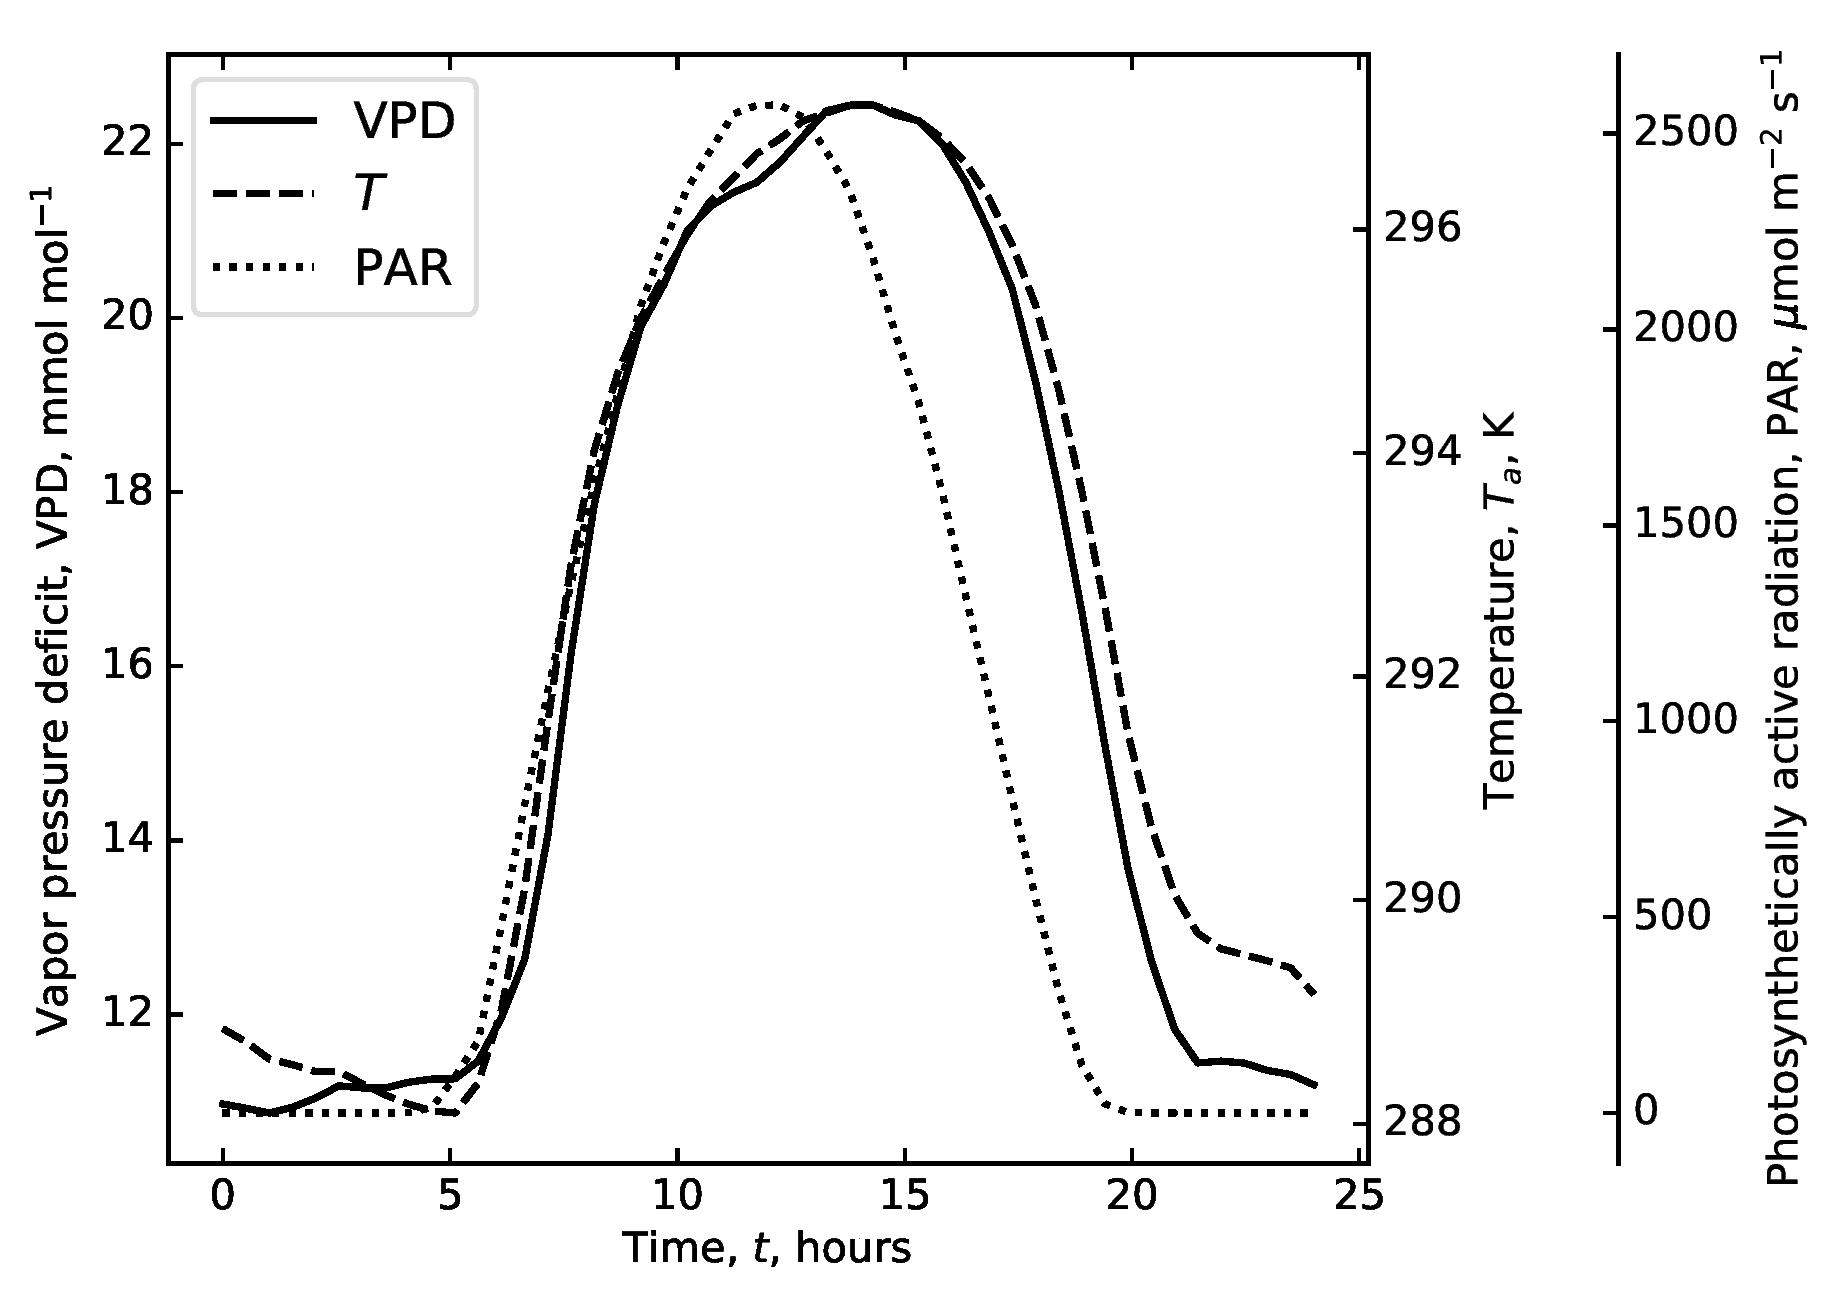
\includegraphics[scale=0.75]{environment.jpg} 
    \end{center}
    \caption{Diurnal trends of vapor pressure deficit (VPD), temperature ($T$), and photosynthetically active radiation (PAR). These are the averaged trends using measurements from the FLUXNET project at the Blodgett forest over 100 days starting from 5-29-2004 (the start of 4-months drought). These trends are repeated for the desired simulation duration.}
    \label{fig:environment}
\end{figure}

% \begin{figure}[h]
%     \begin{center}
%          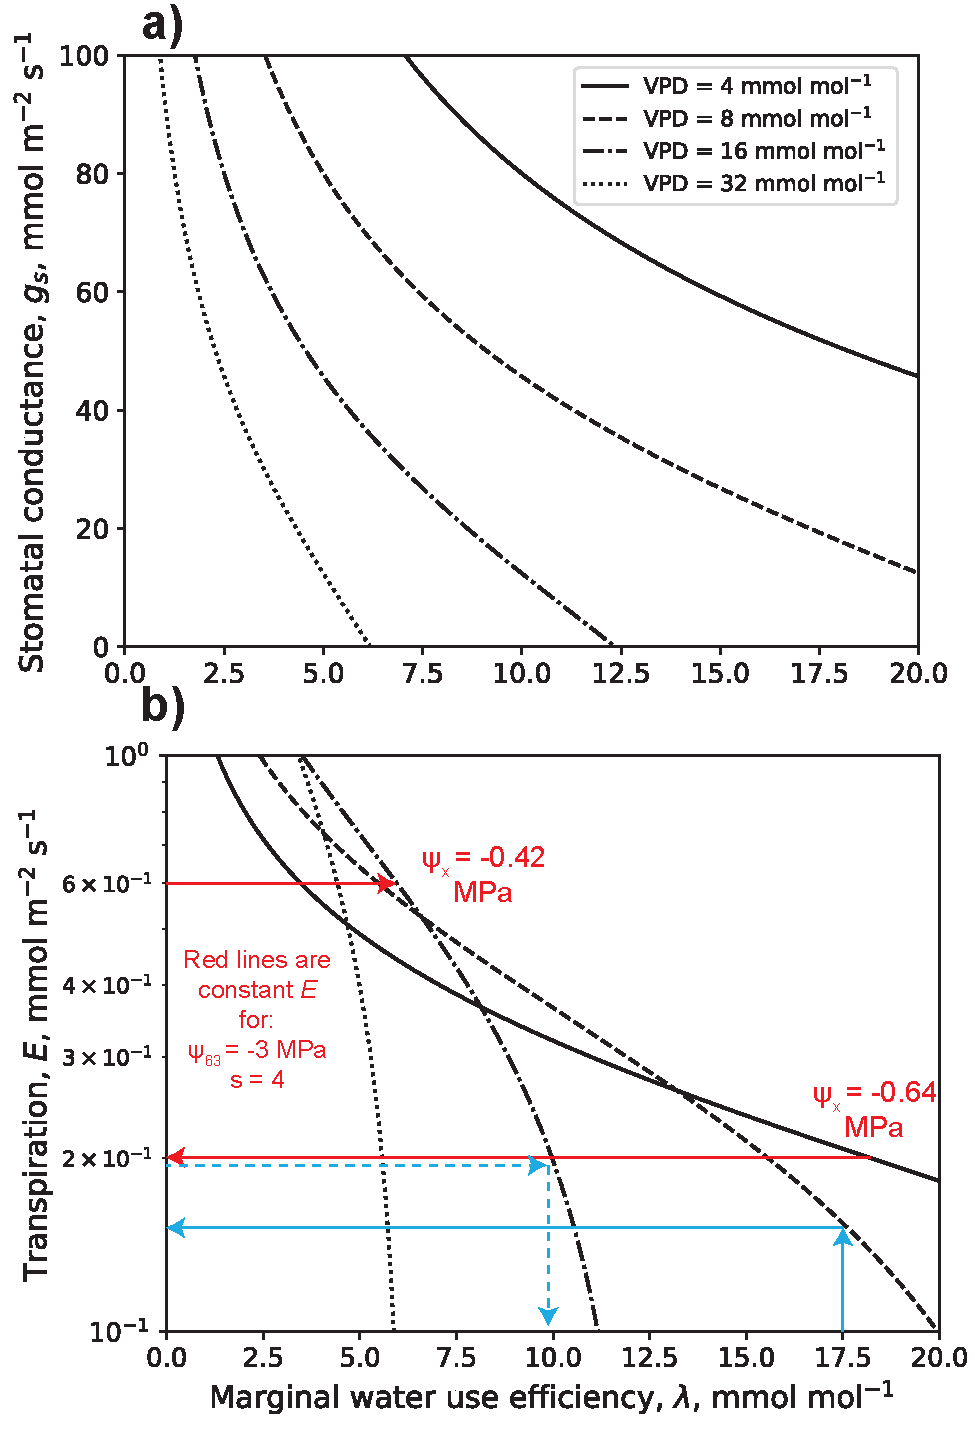
\includegraphics[scale=0.5]{g_E_lam_noon.pdf}   
%     \end{center}
%     \caption{a) Phase space of stomatal conductance $g_s$ vs the marginal water use efficiency $\lambda$ as a result of equation \ref{eqn:control} for different vapor pressure deficits (VPD). Other environmental conditions correspond to those shown in figure \ref{fig:environment} at noon and in table \ref{tab:props}. An increase in VPD or $\lambda$ both decrease $g_s$ with the other kept at constant. b) Transpiration $E$ corresponding to the curves in the phase space in panel a. An increase in $\lambda$ always leads to a decrease in $E$ when VPD is kept constant however the change in $E$ with changing VPD is more nuanced and depends on the value of $\lambda$. The solid blue arrows show how the value of $\lambda$ determines $E$ when transpiration is demand driven. When transpiration is supply limited, the maximum $E$ possible determines $\lambda$ as illustrated by the dashed blue arrows. Red horizontal arrows show the trends in $\lambda$ with changing VPD for supply limited transpiration of a plant with vulnerability curve (VC) parameters $\psi_{63}=-3$ MPa and $s=4$. The upper red arrow, showing constant $E$ at soil water potential $\psi_x = -0.42$ MPa, shows how $\lambda$ increases as the air dries from VPD$=4$ mmol mol$^{-1}$ to VPD$=16$ mmol mol$^{-1}$. The trend reverses as VPD continues increasing to $32$ mmol mol$^{-1}$. At $\psi_x = -0.64$ MPa, the trend in $\lambda$ reverses as shown by the lower red line. One can then trace these $\lambda$ trends to $g_s$ in panel a and infer magnitudes of midday stomatal closure and day to day $g_s$ sensitivity to drought.}
%     \label{fig:gs_E_lam}
% \end{figure}

\begin{figure}[h]
    \begin{center}
         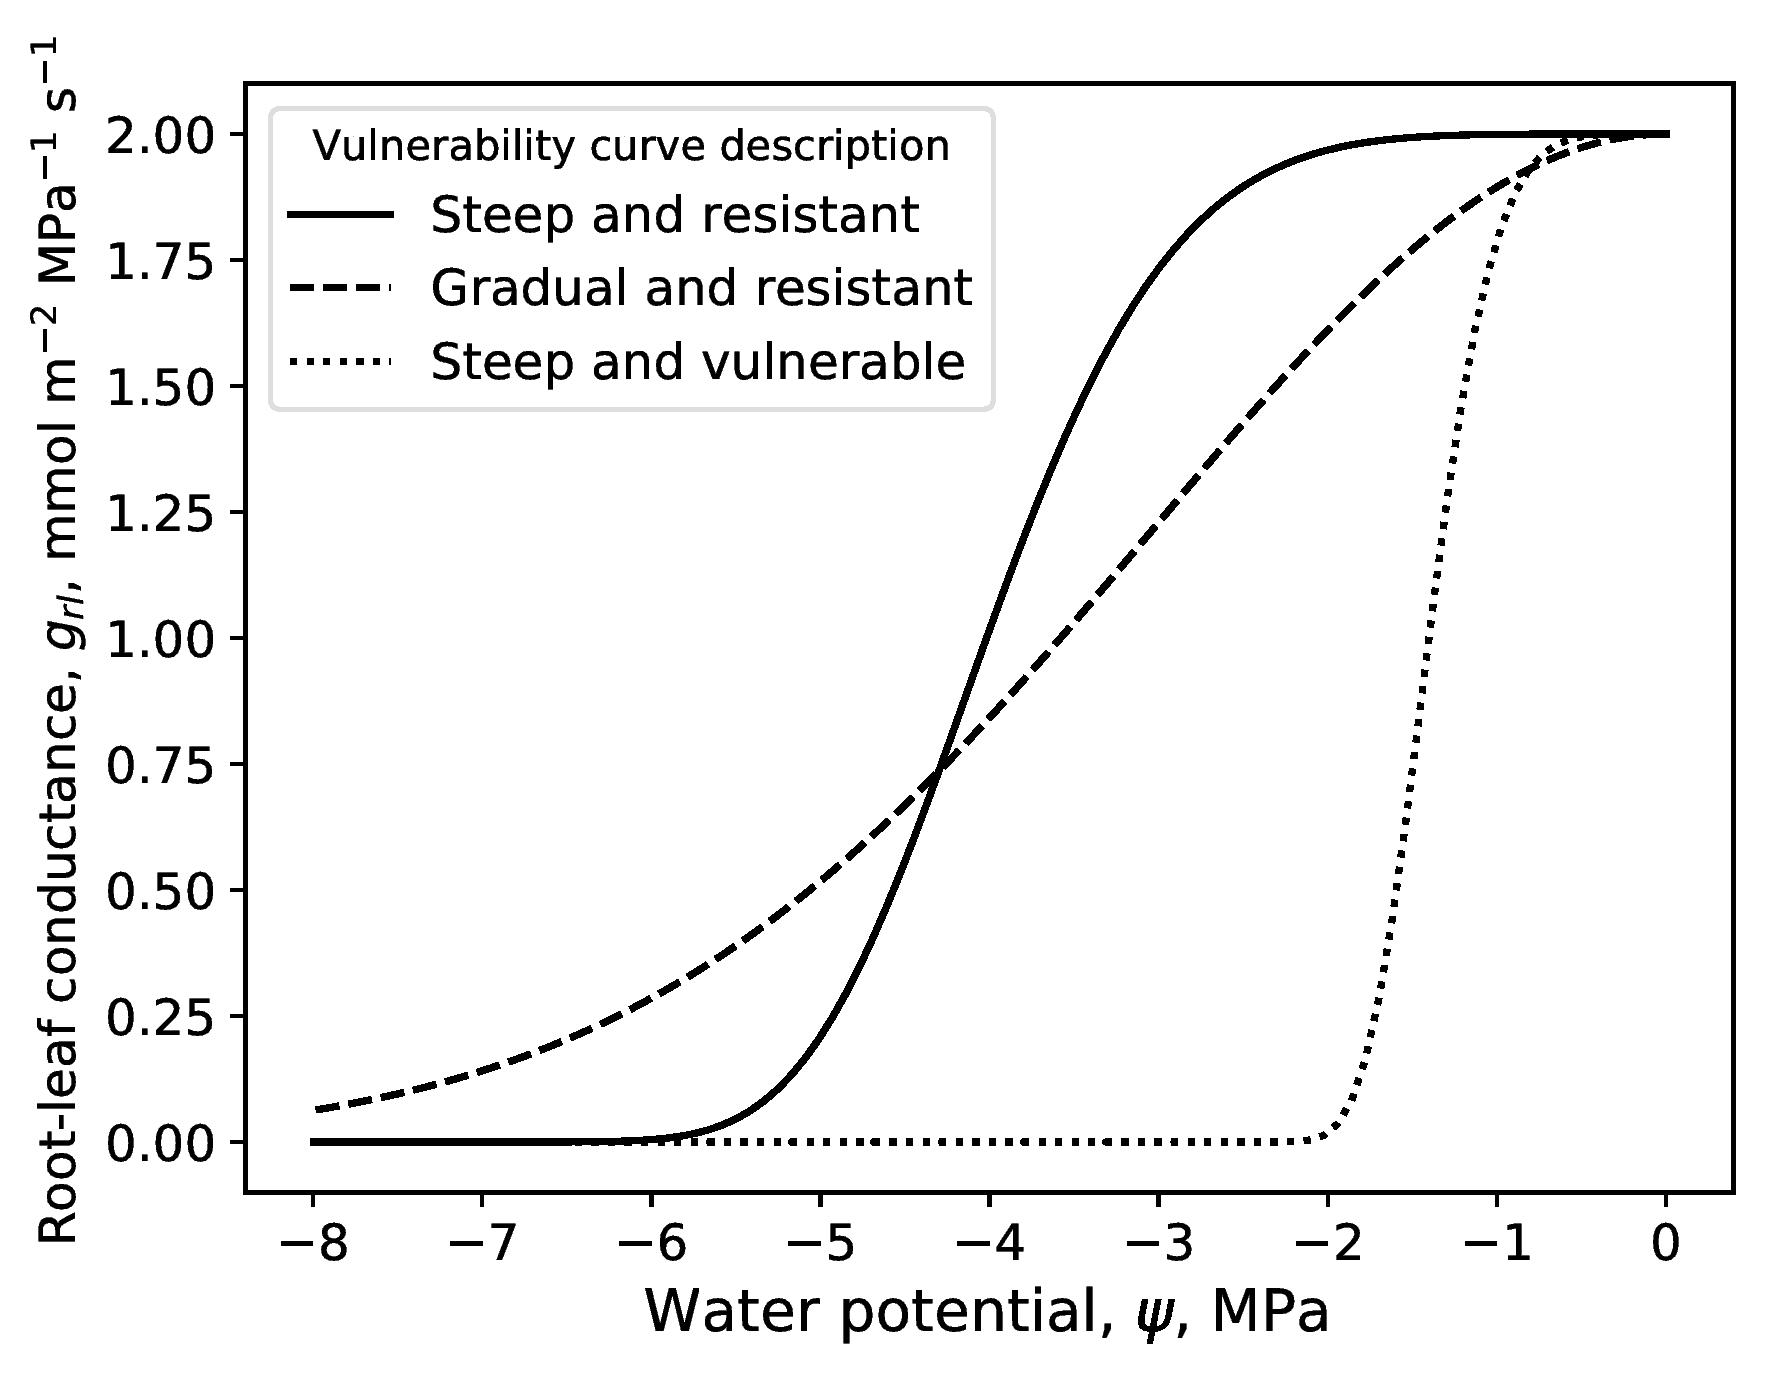
\includegraphics[scale=0.75]{grl.jpg}   
    \end{center}
    \caption{Loss of conductance curves for the three plants simulated throughout this work. The steep and resistant vulnerability curve has parameters $\psi_{63} = -4.3$ MPa, $s=5.4$, and $g_{rl,max} = 2$ mmol m$^{-2}$ MPa$^{-1}$ s$^{-1}$, the gradual and resistant has $\psi_{63} = -4.3$ MPa, $s=2$, and $g_{rl,max} = 2$ mmol m$^{-2}$ MPa$^{-1}$ s$^{-1}$, and the steep and vulnerable has $\psi_{63} = -1.5$ MPa, $s=5.4$, and $g_{rl,max} = 2$ mmol m$^{-2}$ MPa$^{-1}$ s$^{-1}$.}
    \label{fig:grl}
\end{figure}

\begin{figure}[h]
    \begin{center}
        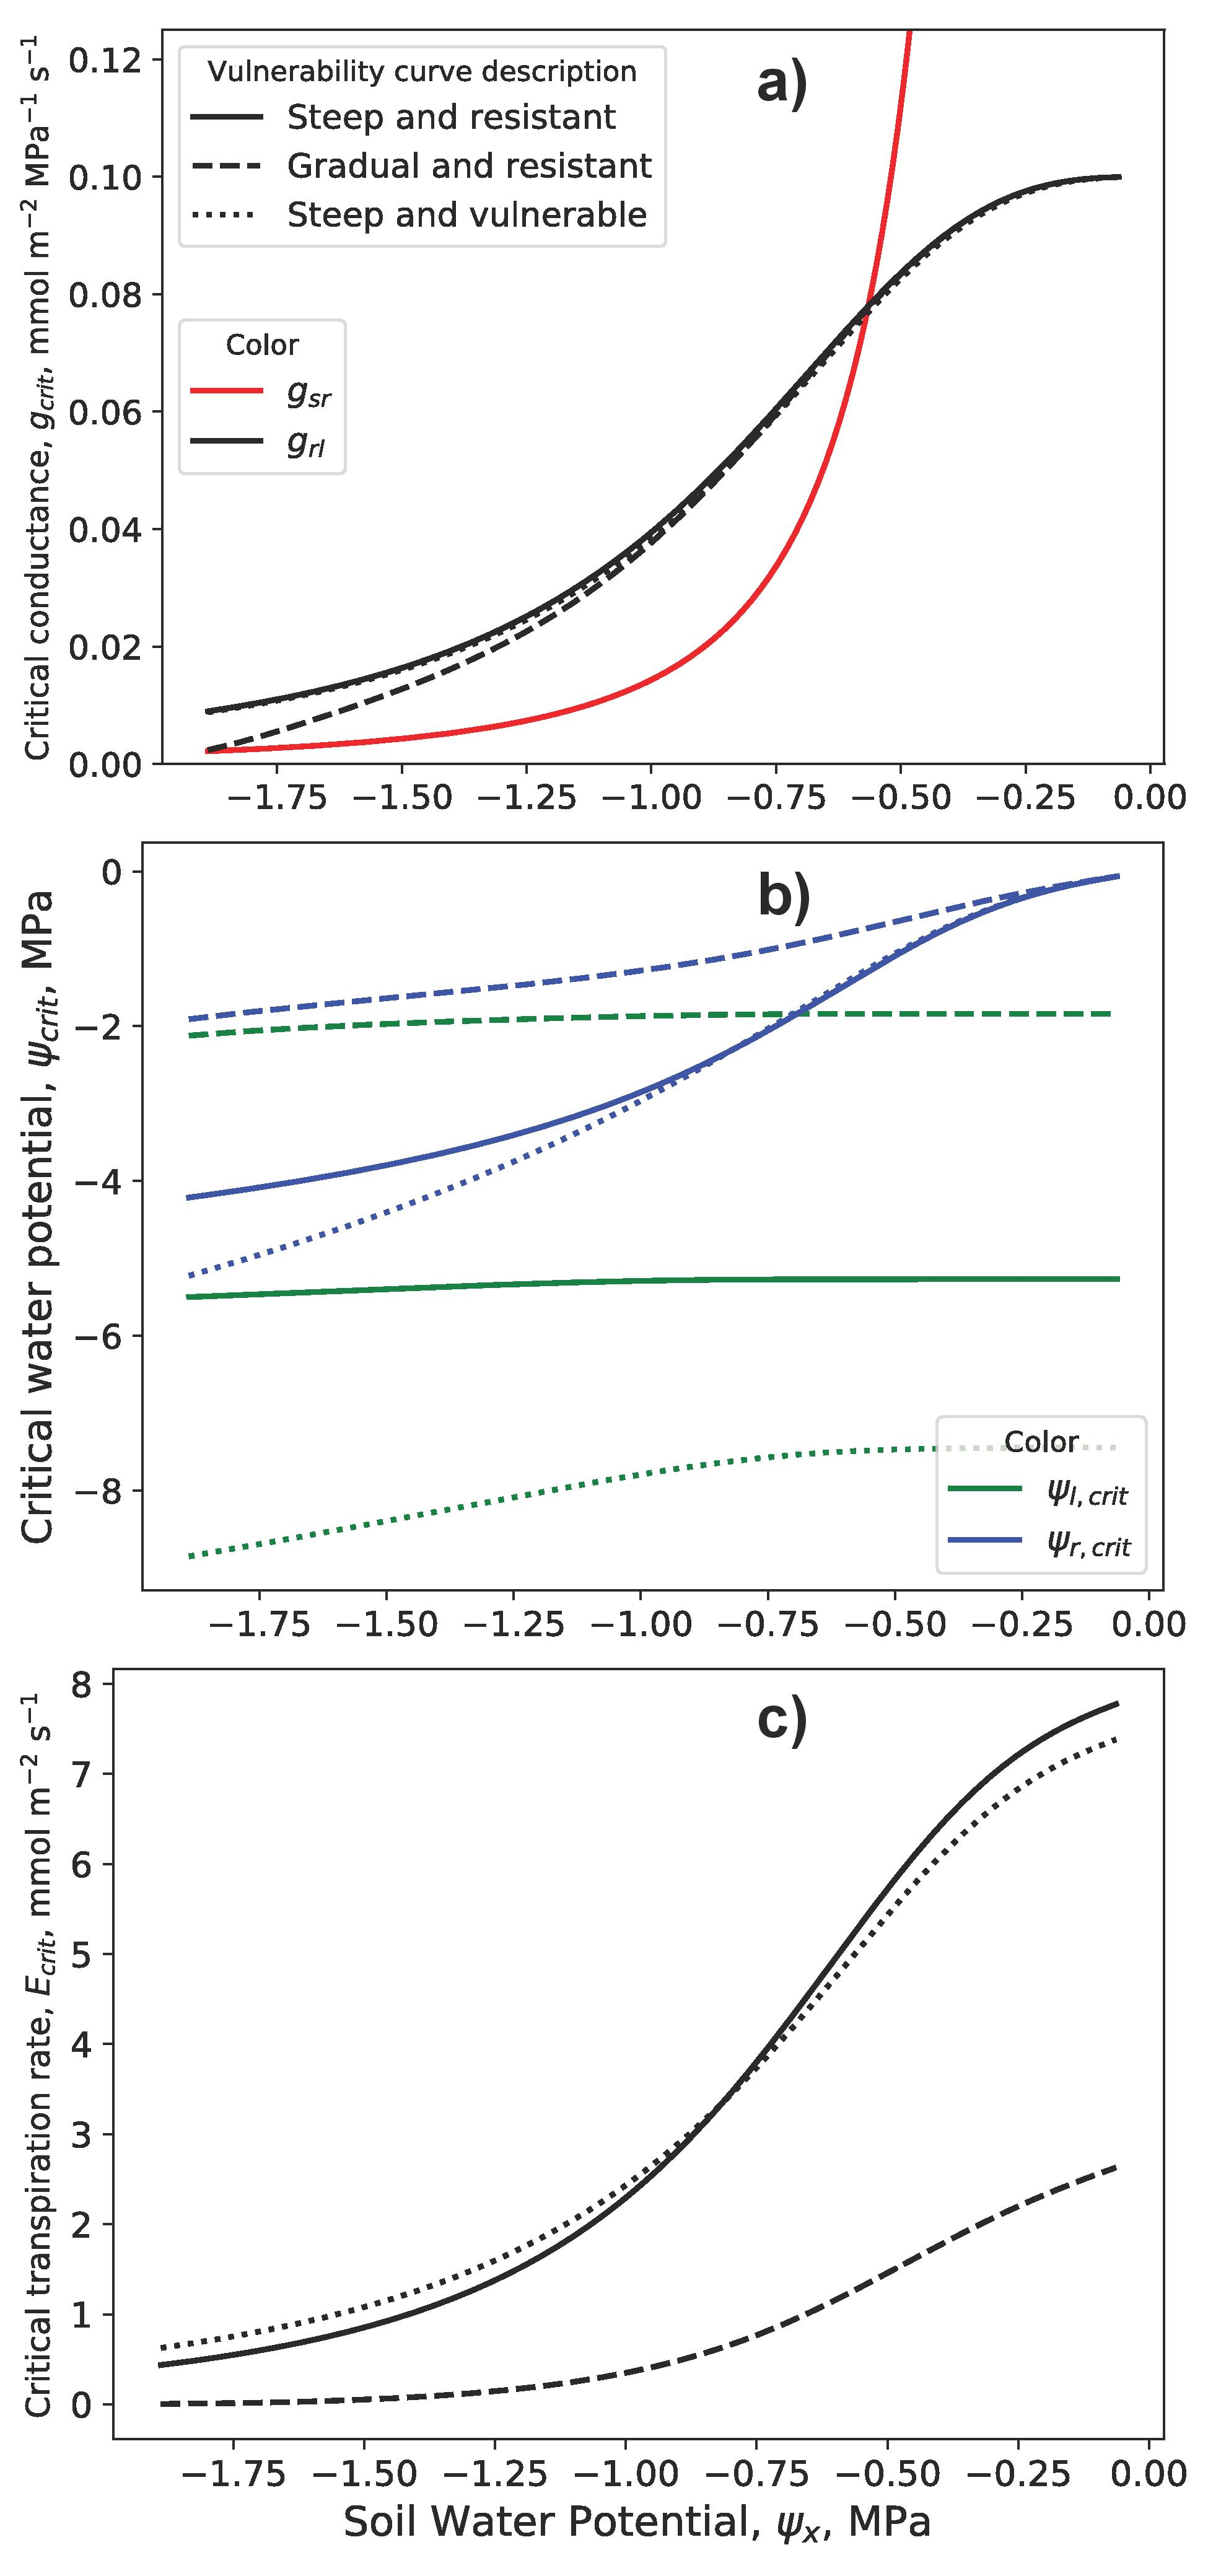
\includegraphics[scale=0.5]{g_psi_E_psix.jpg}
    \end{center}
    \caption{a) Soil to root conductance of the rhizosphere ($g_{sr}$) and root to leaf conductance of the plant ($g_{rl}$) that critical transpiration rate $E_{crit}$ for difference soil water potentials $\psi_x$. Soil is sandy loam and particular hydraulic parameters are shown in table \ref{tab:props}. Three vulnerability curve (VC) examples give different $g_{rl}$ trends. The VCs are described and plotted in figure \ref{fig:grl}. b) Critical root and leaf water potentials ($\psi_r$ and $\psi_l$, respectively) for the three VCs and for the particular soil type. The gradual and resistant VC ($s=2$) can maintain a gap between $\psi_r$ and $\psi_l$ as $\psi_x$ decreases unlike the other two VCs. c) The critical transpiration rates $E_{crit}$ for the three VCs. Details on how these curves were derived are available in the main text}
    \label{fig:gmax_Emax_psix}
\end{figure}

\begin{figure}[h]
    \begin{center}
         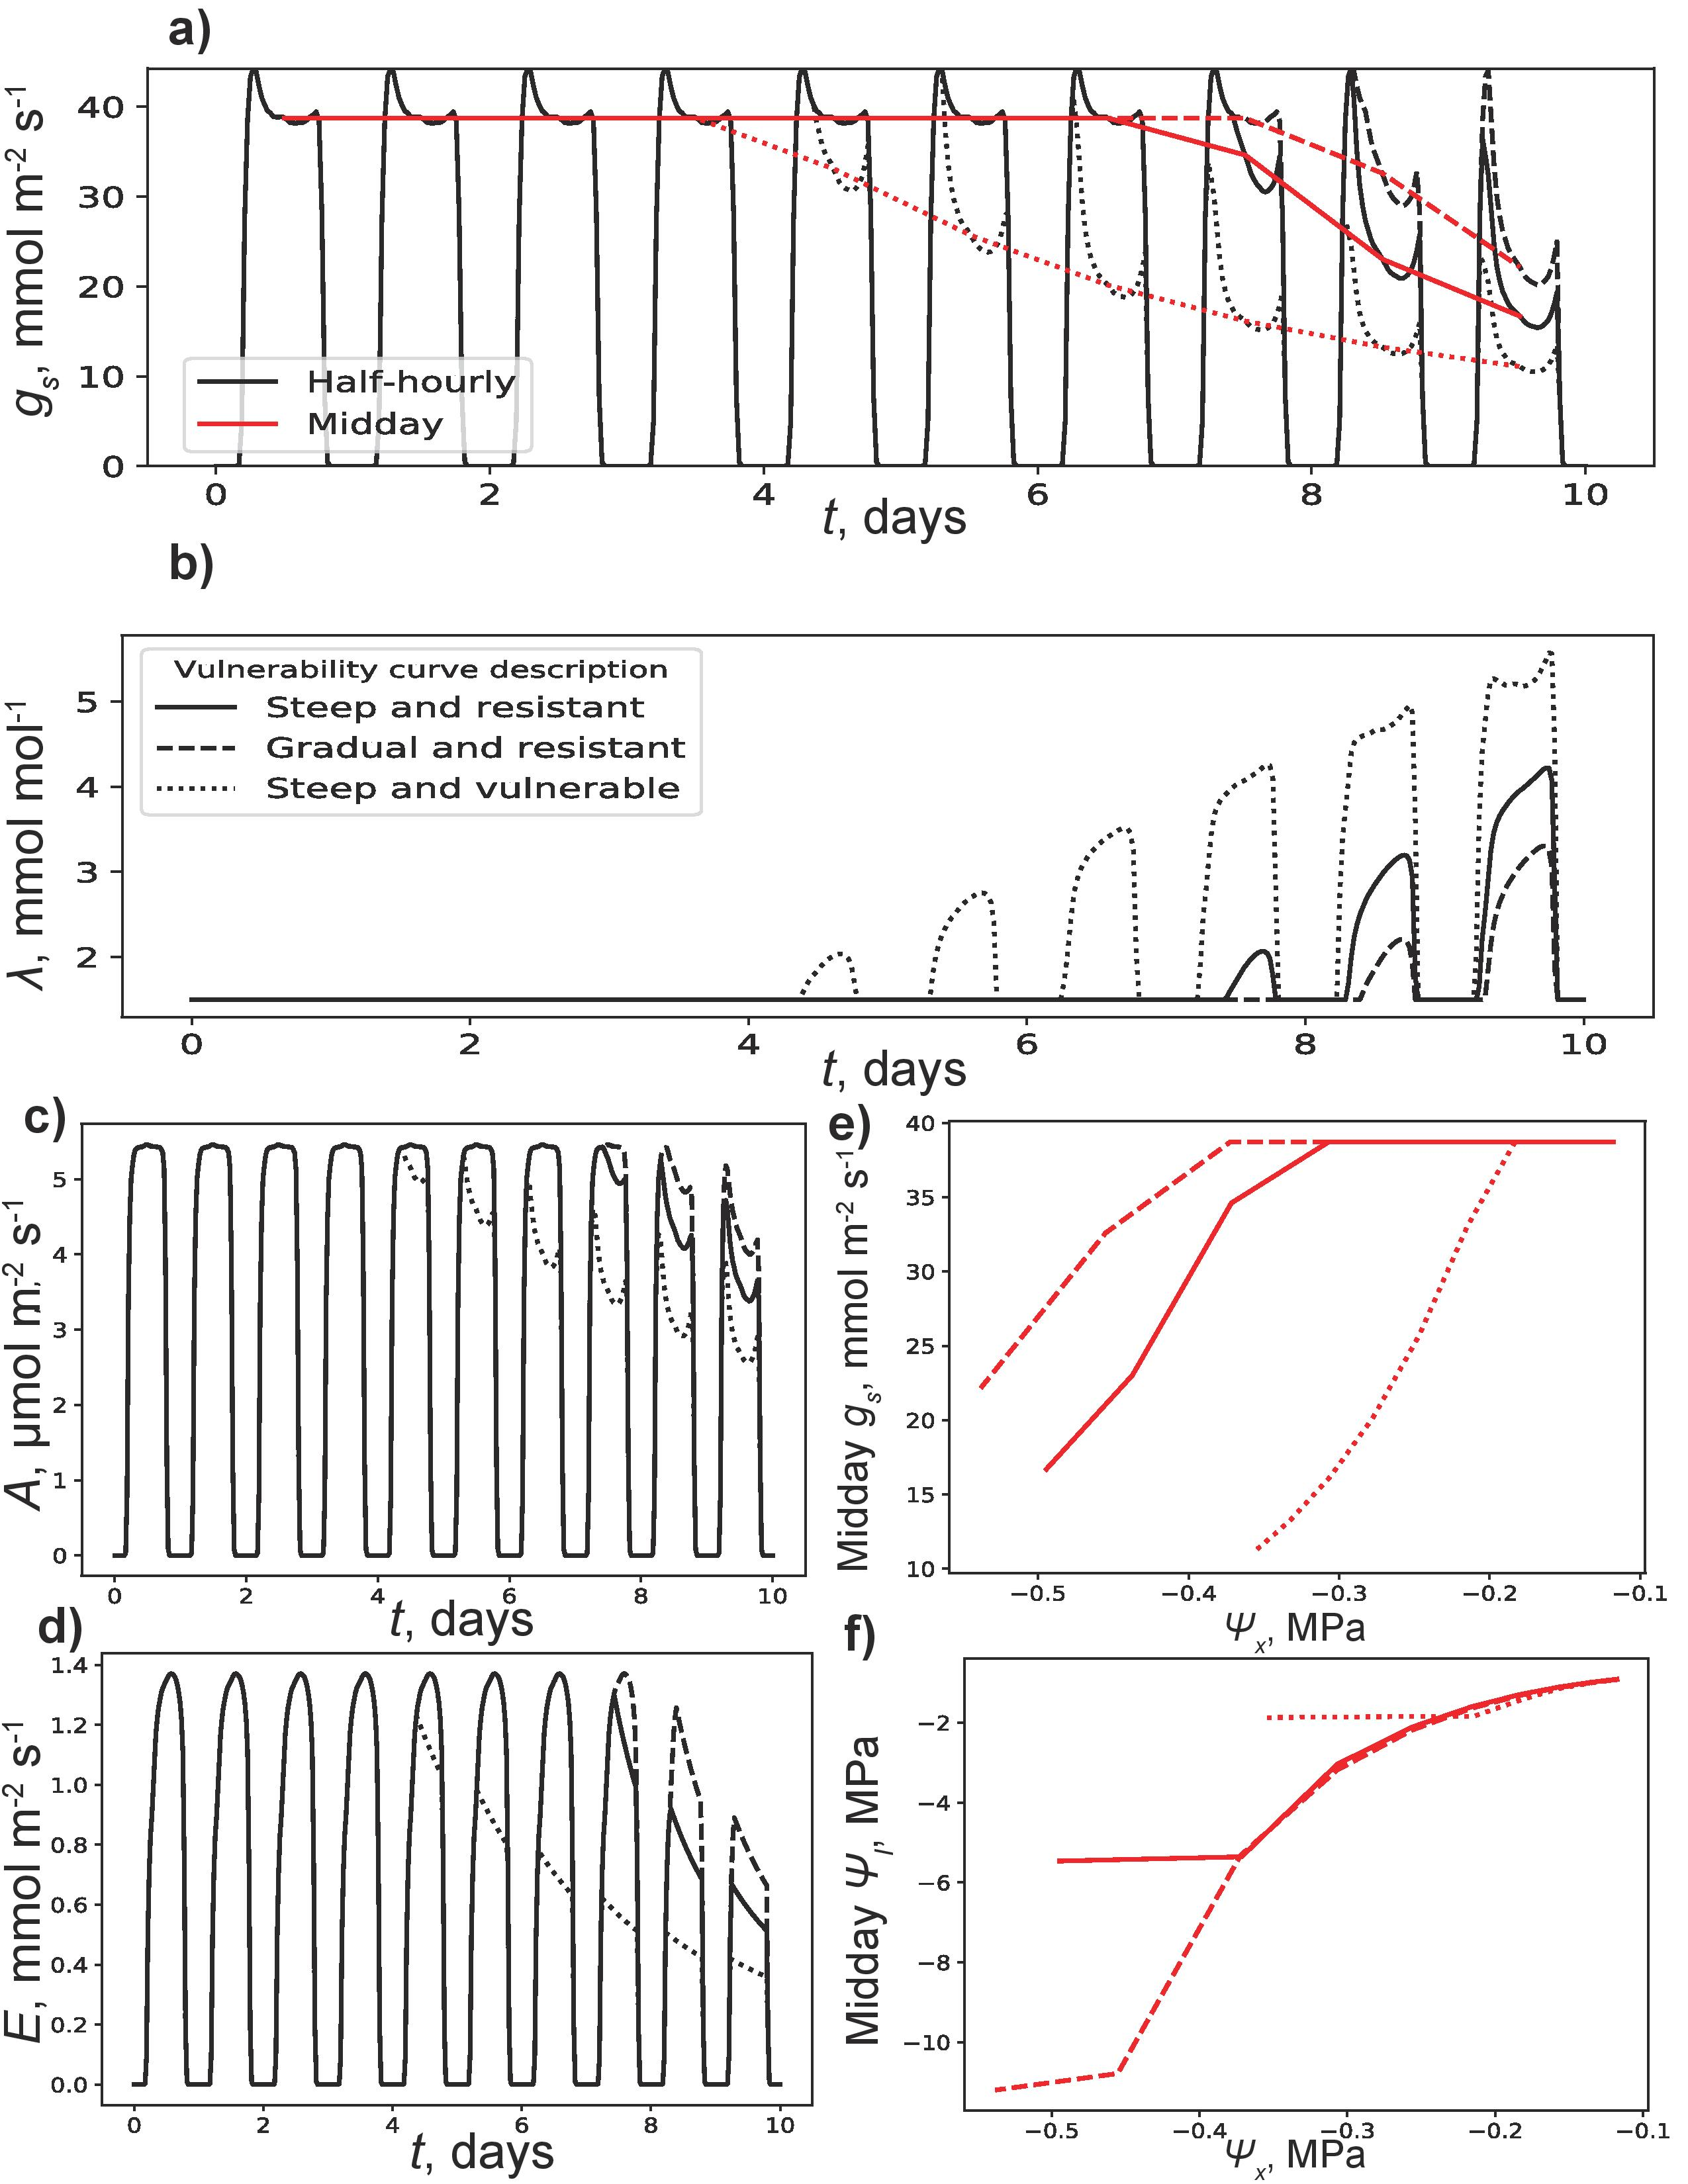
\includegraphics[scale=0.65]{WUS_no_comp.jpg} 
    \end{center}
    \caption{Results of a simulation where at time $t=0$, soil moisture $x(0) =0.25$. There are no competitive soil water users and the terminal marginal water use efficiency is set at $\lambda(10) = 1.6$ mmol mol$^{-1}$. a) Half-hourly (black) and midday (red) trends of stomatal conductance ($g_s$) with $t$ and b) $\lambda$ with $t$. Trends are shown for the three vulnerability curves (VCs) described and plotted in figure \ref{fig:grl}. Other plant and soil parameters are listed in the table \ref{tab:props}. c) Carbon assimilation rate ($A$) and d) transpiration rate ($E$) with $t$. e) Midday $g_s$ and f) midday leaf water potential $\psi_l$ with soil water potential $\psi_x$.}
    \label{fig:WUS_no_comp}
\end{figure}

\begin{figure}[h]
    \begin{center}
         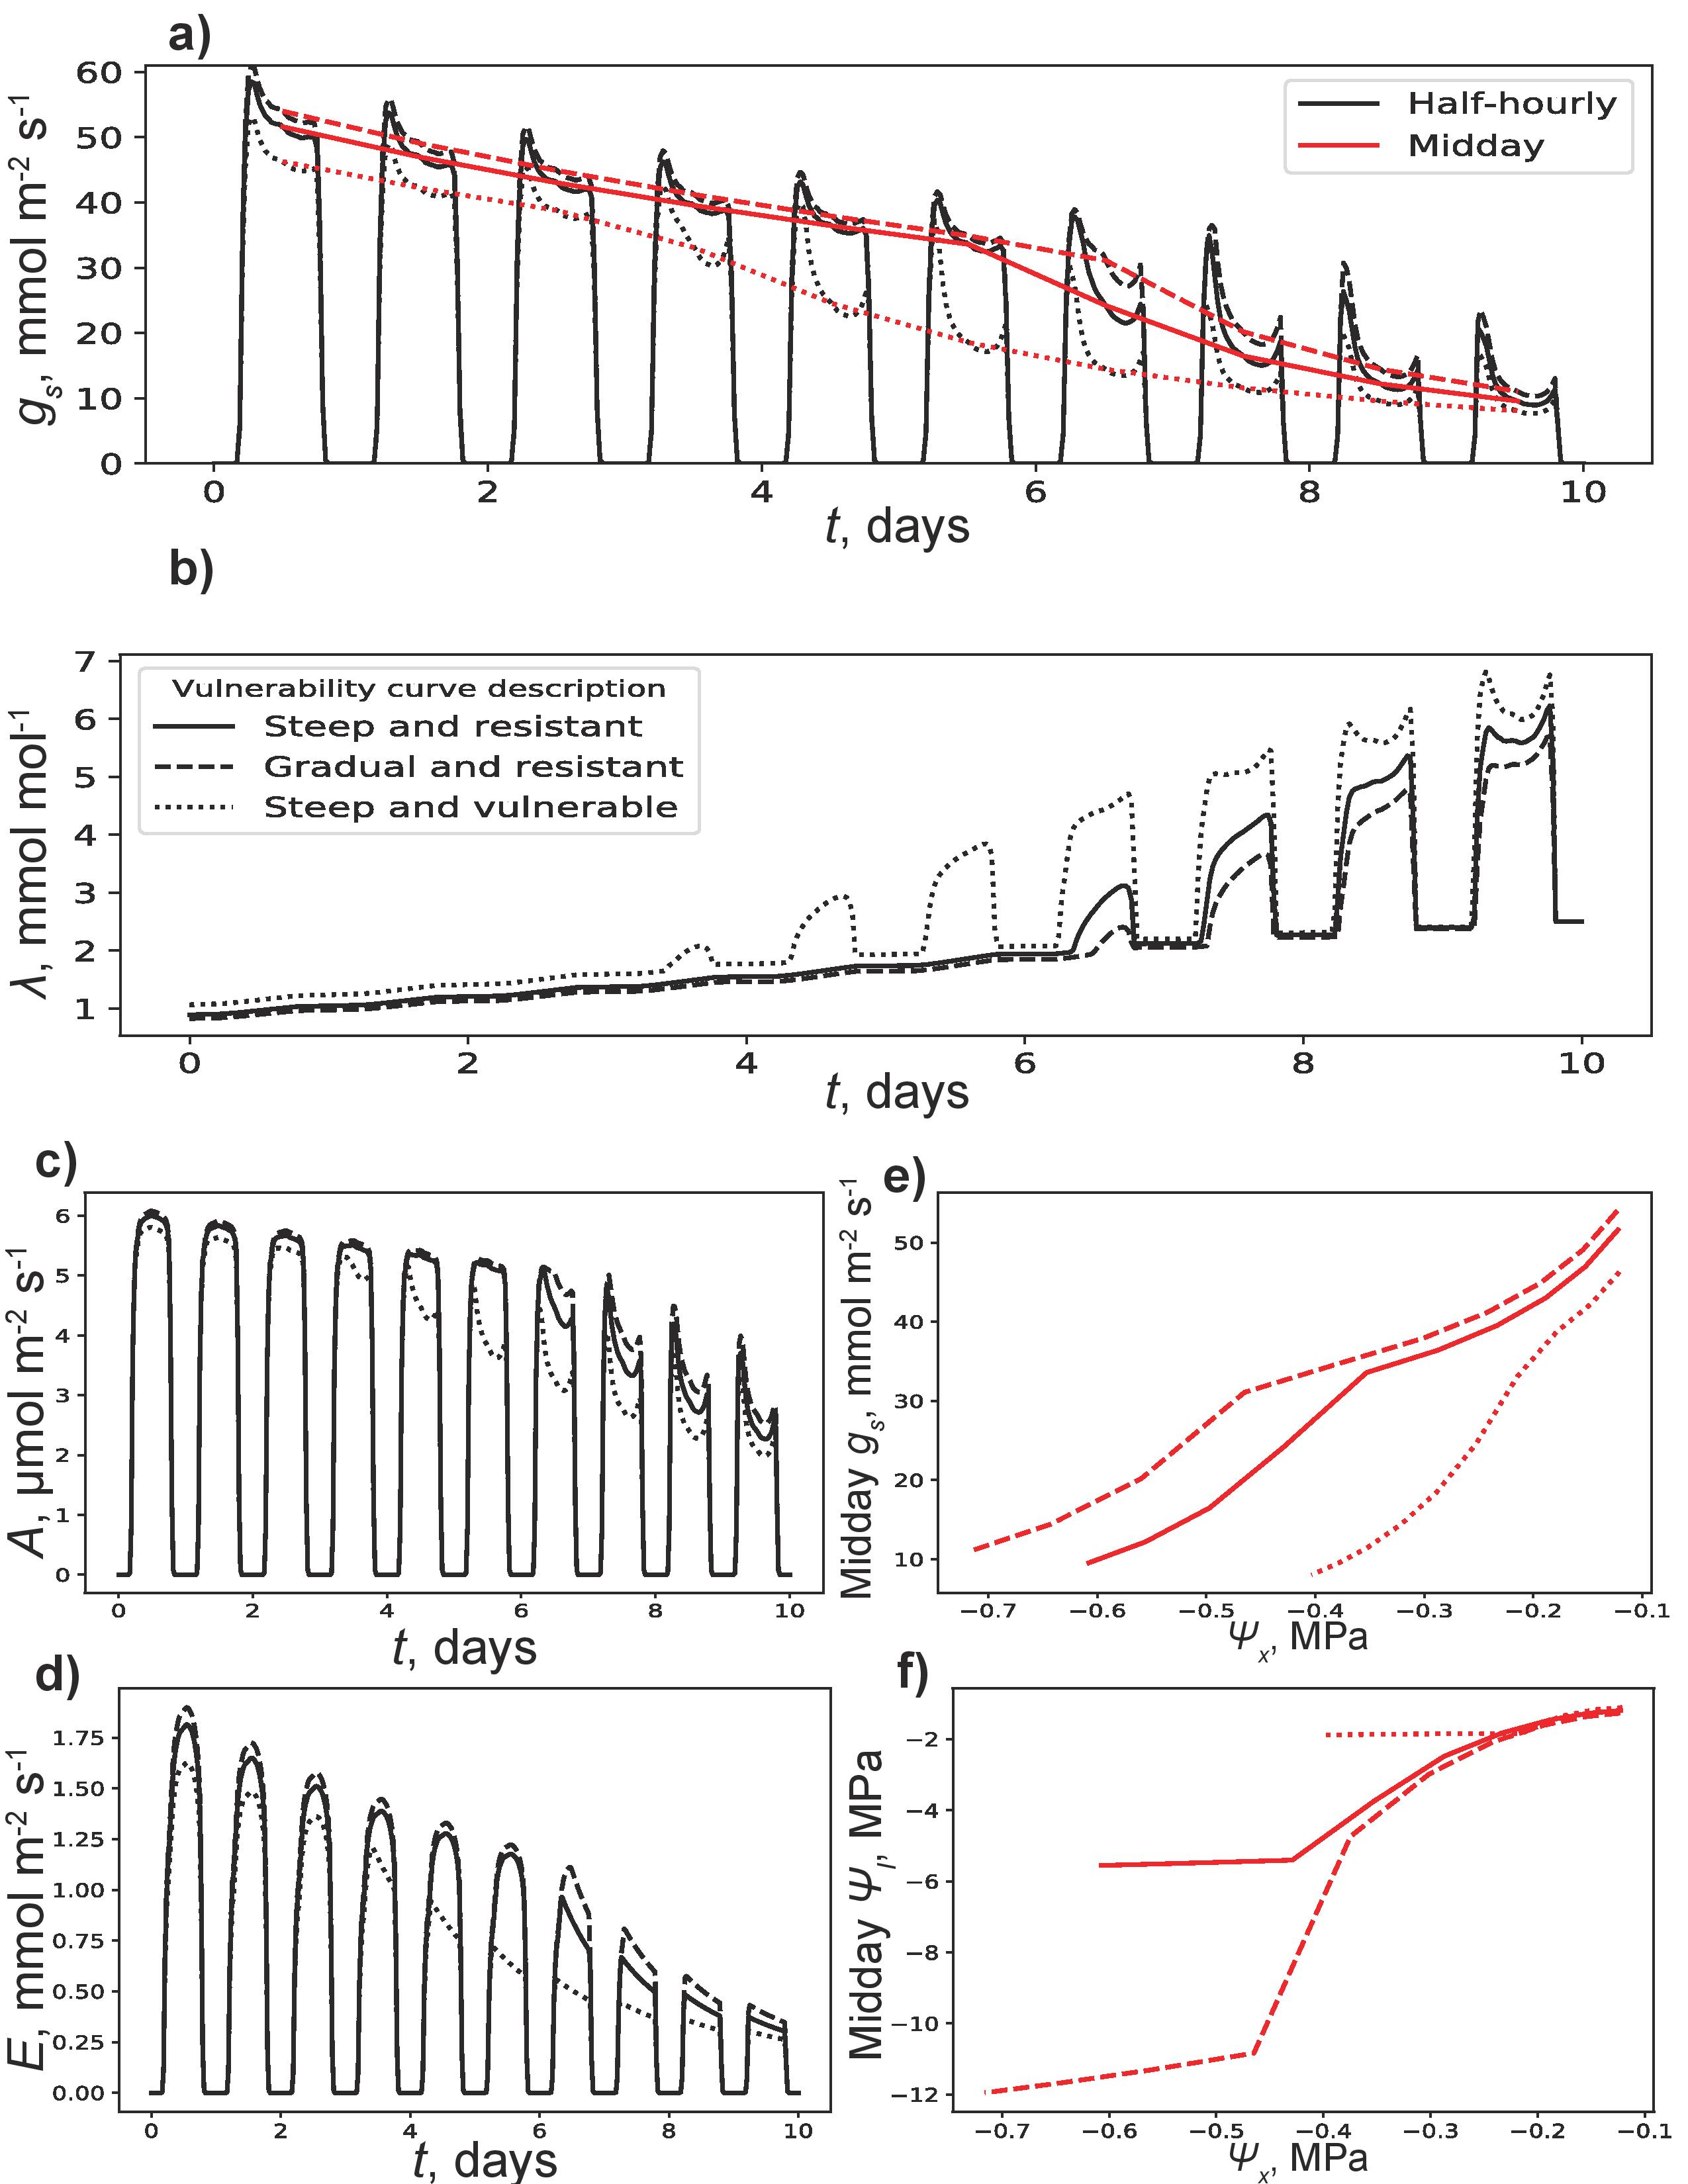
\includegraphics[scale=0.65]{WUS_comp.jpg}   
    \end{center}
    \caption{Results of a simulation where at time $t=0$, soil moisture $x(0) =0.25$. The terminal marginal water use efficiency is set at $\lambda(10) = 2.5$ mmol mol$^{-1}$. The competitive water sinks are soil free drainage and competing plants with similar vulnerability curves (VCs) and water use strategy (WUS) to those modeled. The competing plants have access to only 20\% of the root zone water of each modeled plant. a) Half-hourly (black) and midday (red) trends of stomatal conductance ($g_s$) with $t$ and b) $\lambda$ with $t$. Trends are shown for the three vulnerability curves (VCs) described and plotted in figure \ref{fig:grl}. Other plant and soil parameters are listed in the table \ref{tab:props}. c) Carbon assimilation rate ($A$) and d) transpiration rate ($E$) with $t$. e) Midday $g_s$ and f) Midday leaf water potential $\psi_l$ with soil water potential $\psi_x$.}
    \label{fig:WUS_comp}
\end{figure}

\begin{figure}[h]
    \begin{center}
         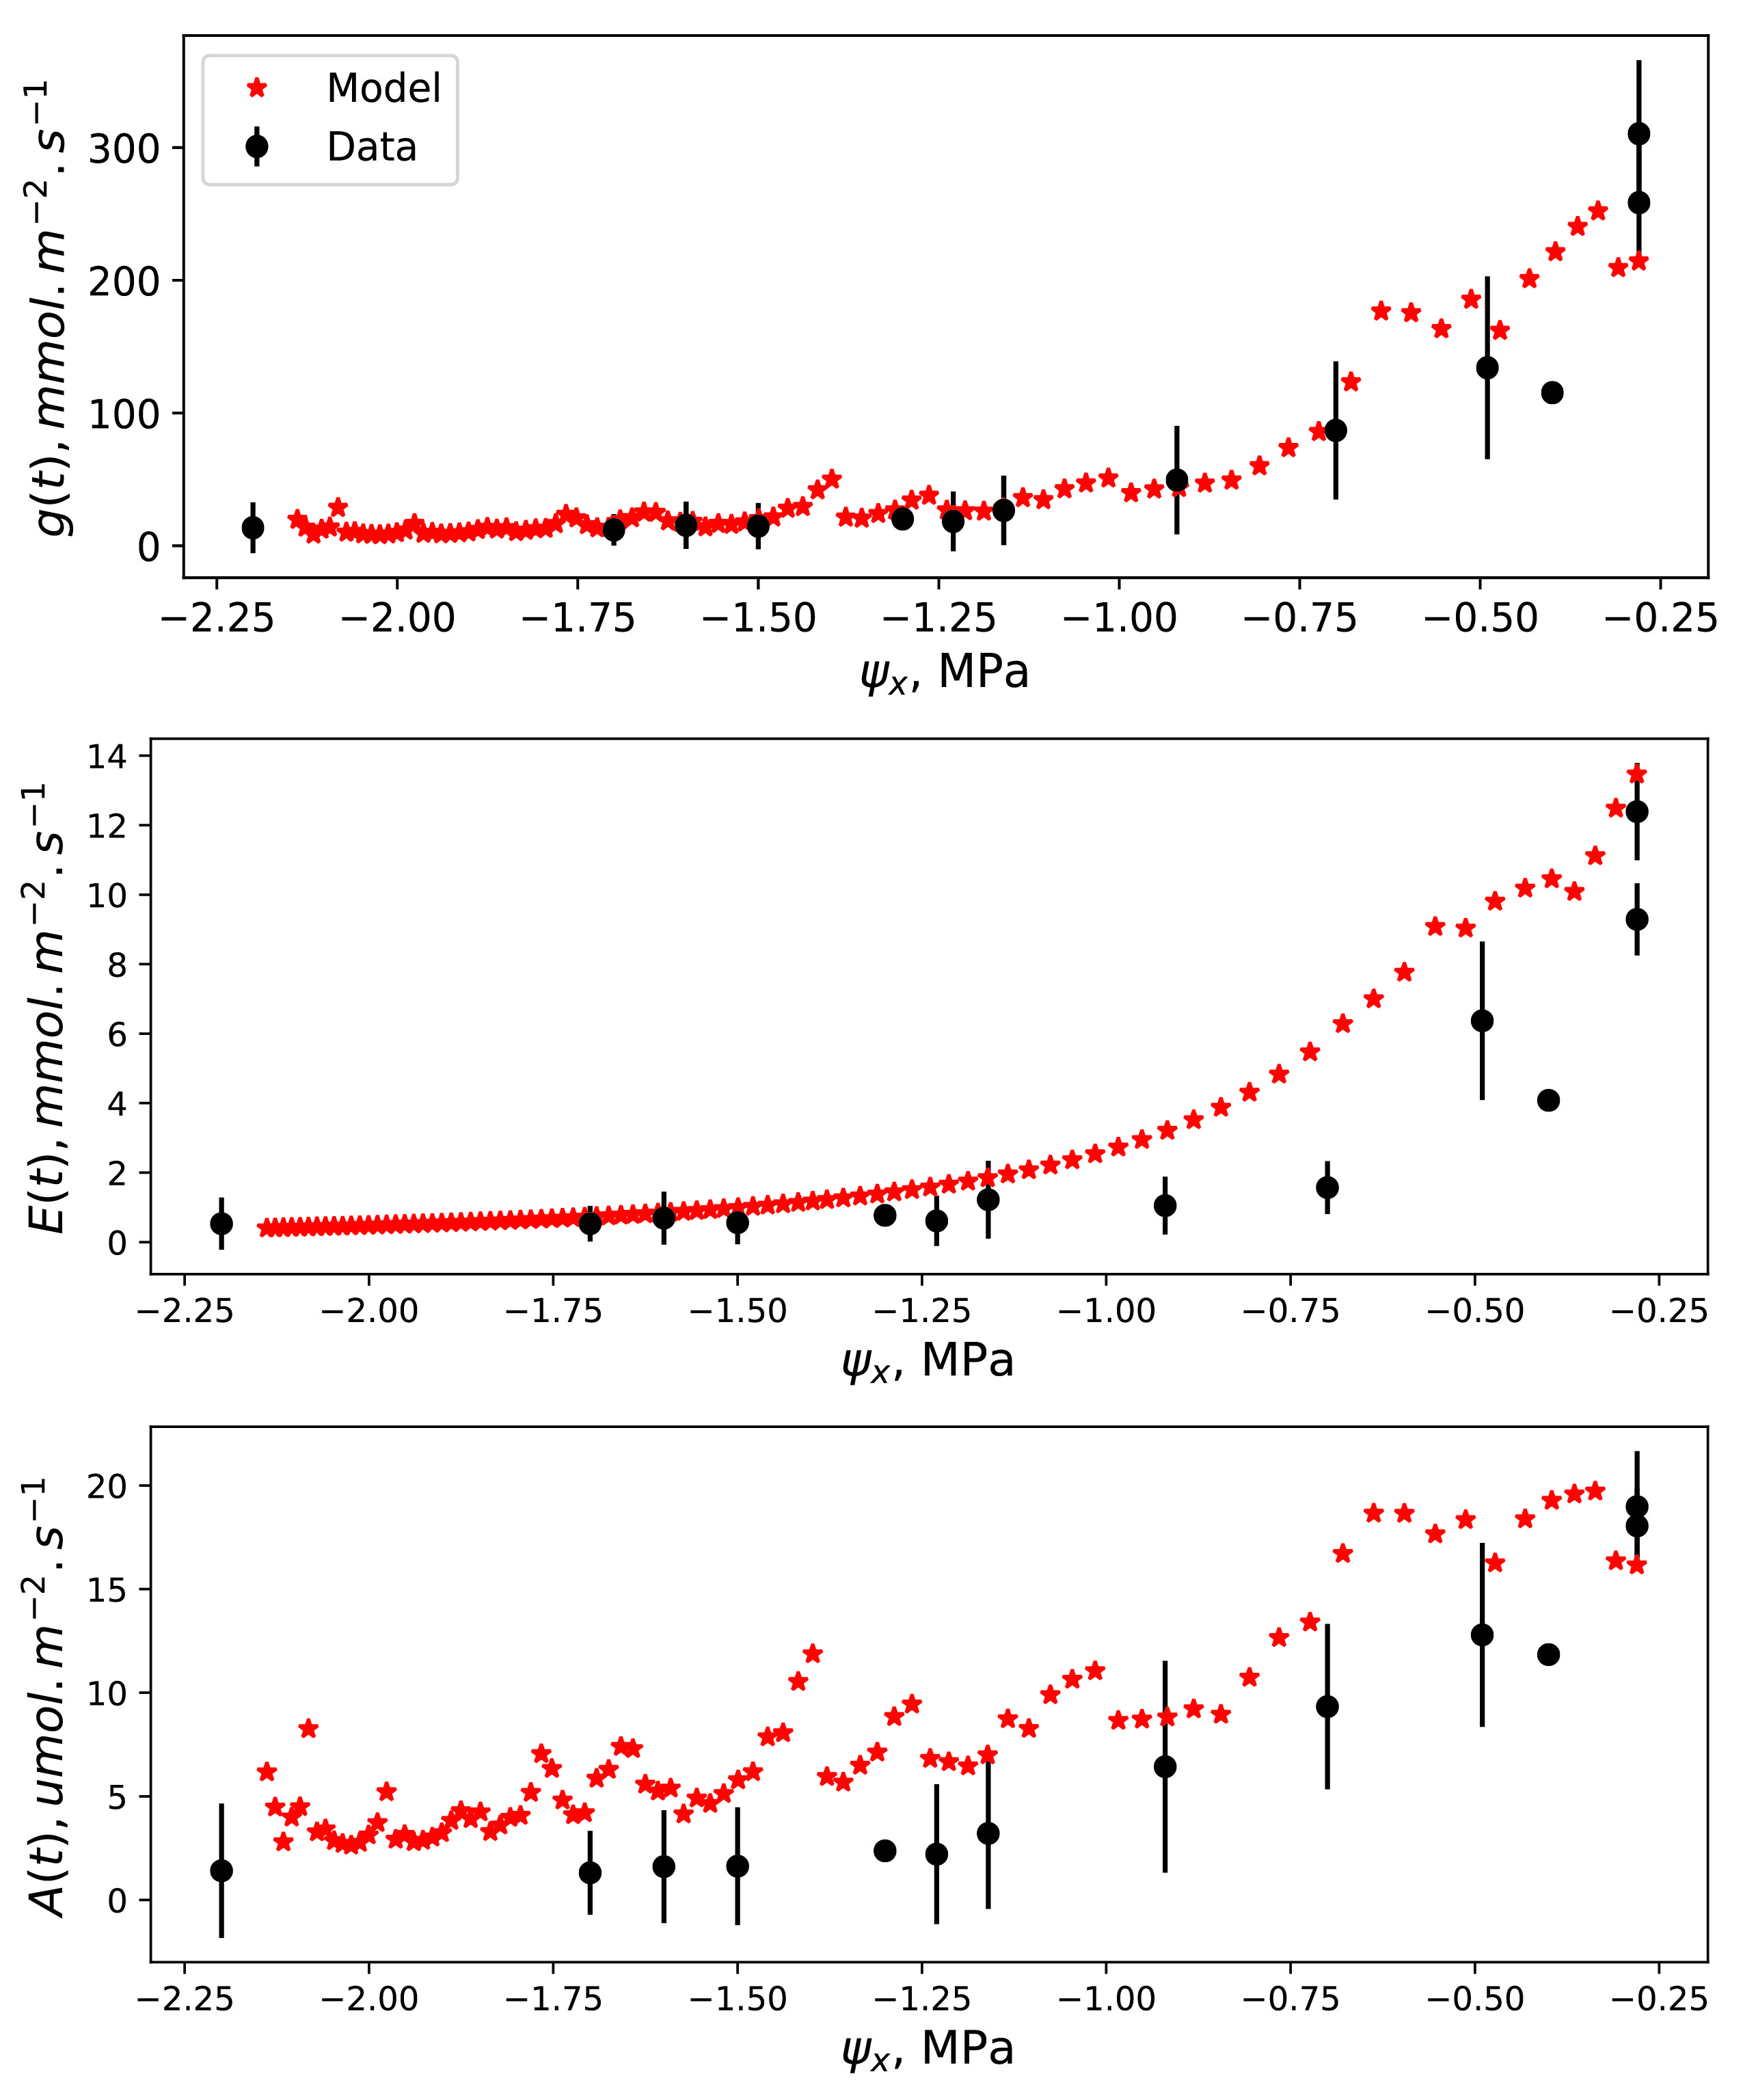
\includegraphics[scale=0.16]{Data_Model.jpg}   
    \end{center}
    \caption{Comparison of model results with the experimental data of \citep{venturas_2018}. Top to bottom are the stomatal conductance per leaf area, transpiration rate per leaf area, and the carbon assimilation rate per leaf area. The atmospheric variables were those measured during the experiment and available in the aforementioned publication. The vulnerability curve used was that of aspen: $\psi_{63} = -3.6$ MPa, $s=1.6$, and $g_{rl,max} = 27$ mmol m$^{-2}$ MPa$^{-1}$ s$^{-1}$ per leaf area. LAI is 0.15, the average value for the severe drought experiment in \citep{venturas_2018}. $V_{max} = 120$ $\mu$mol m$^{-2}$ s$^{-1}$ and $J_{max} = 160$ $\mu$mol m$^{-2}$ s$^{-1}$ at a leaf temperature of 25 degrees celsius. The supply limited regime starts at $\psi_x = -0.55$ MPa. Black vertical lines are the confidence intervals of the measurements computed as $1.96\, \text{SD}/\sqrt{n}$ where SD is the standard deviation.} 
    \label{fig:data_model}
\end{figure}

\begin{figure}[h]
    \begin{center}
         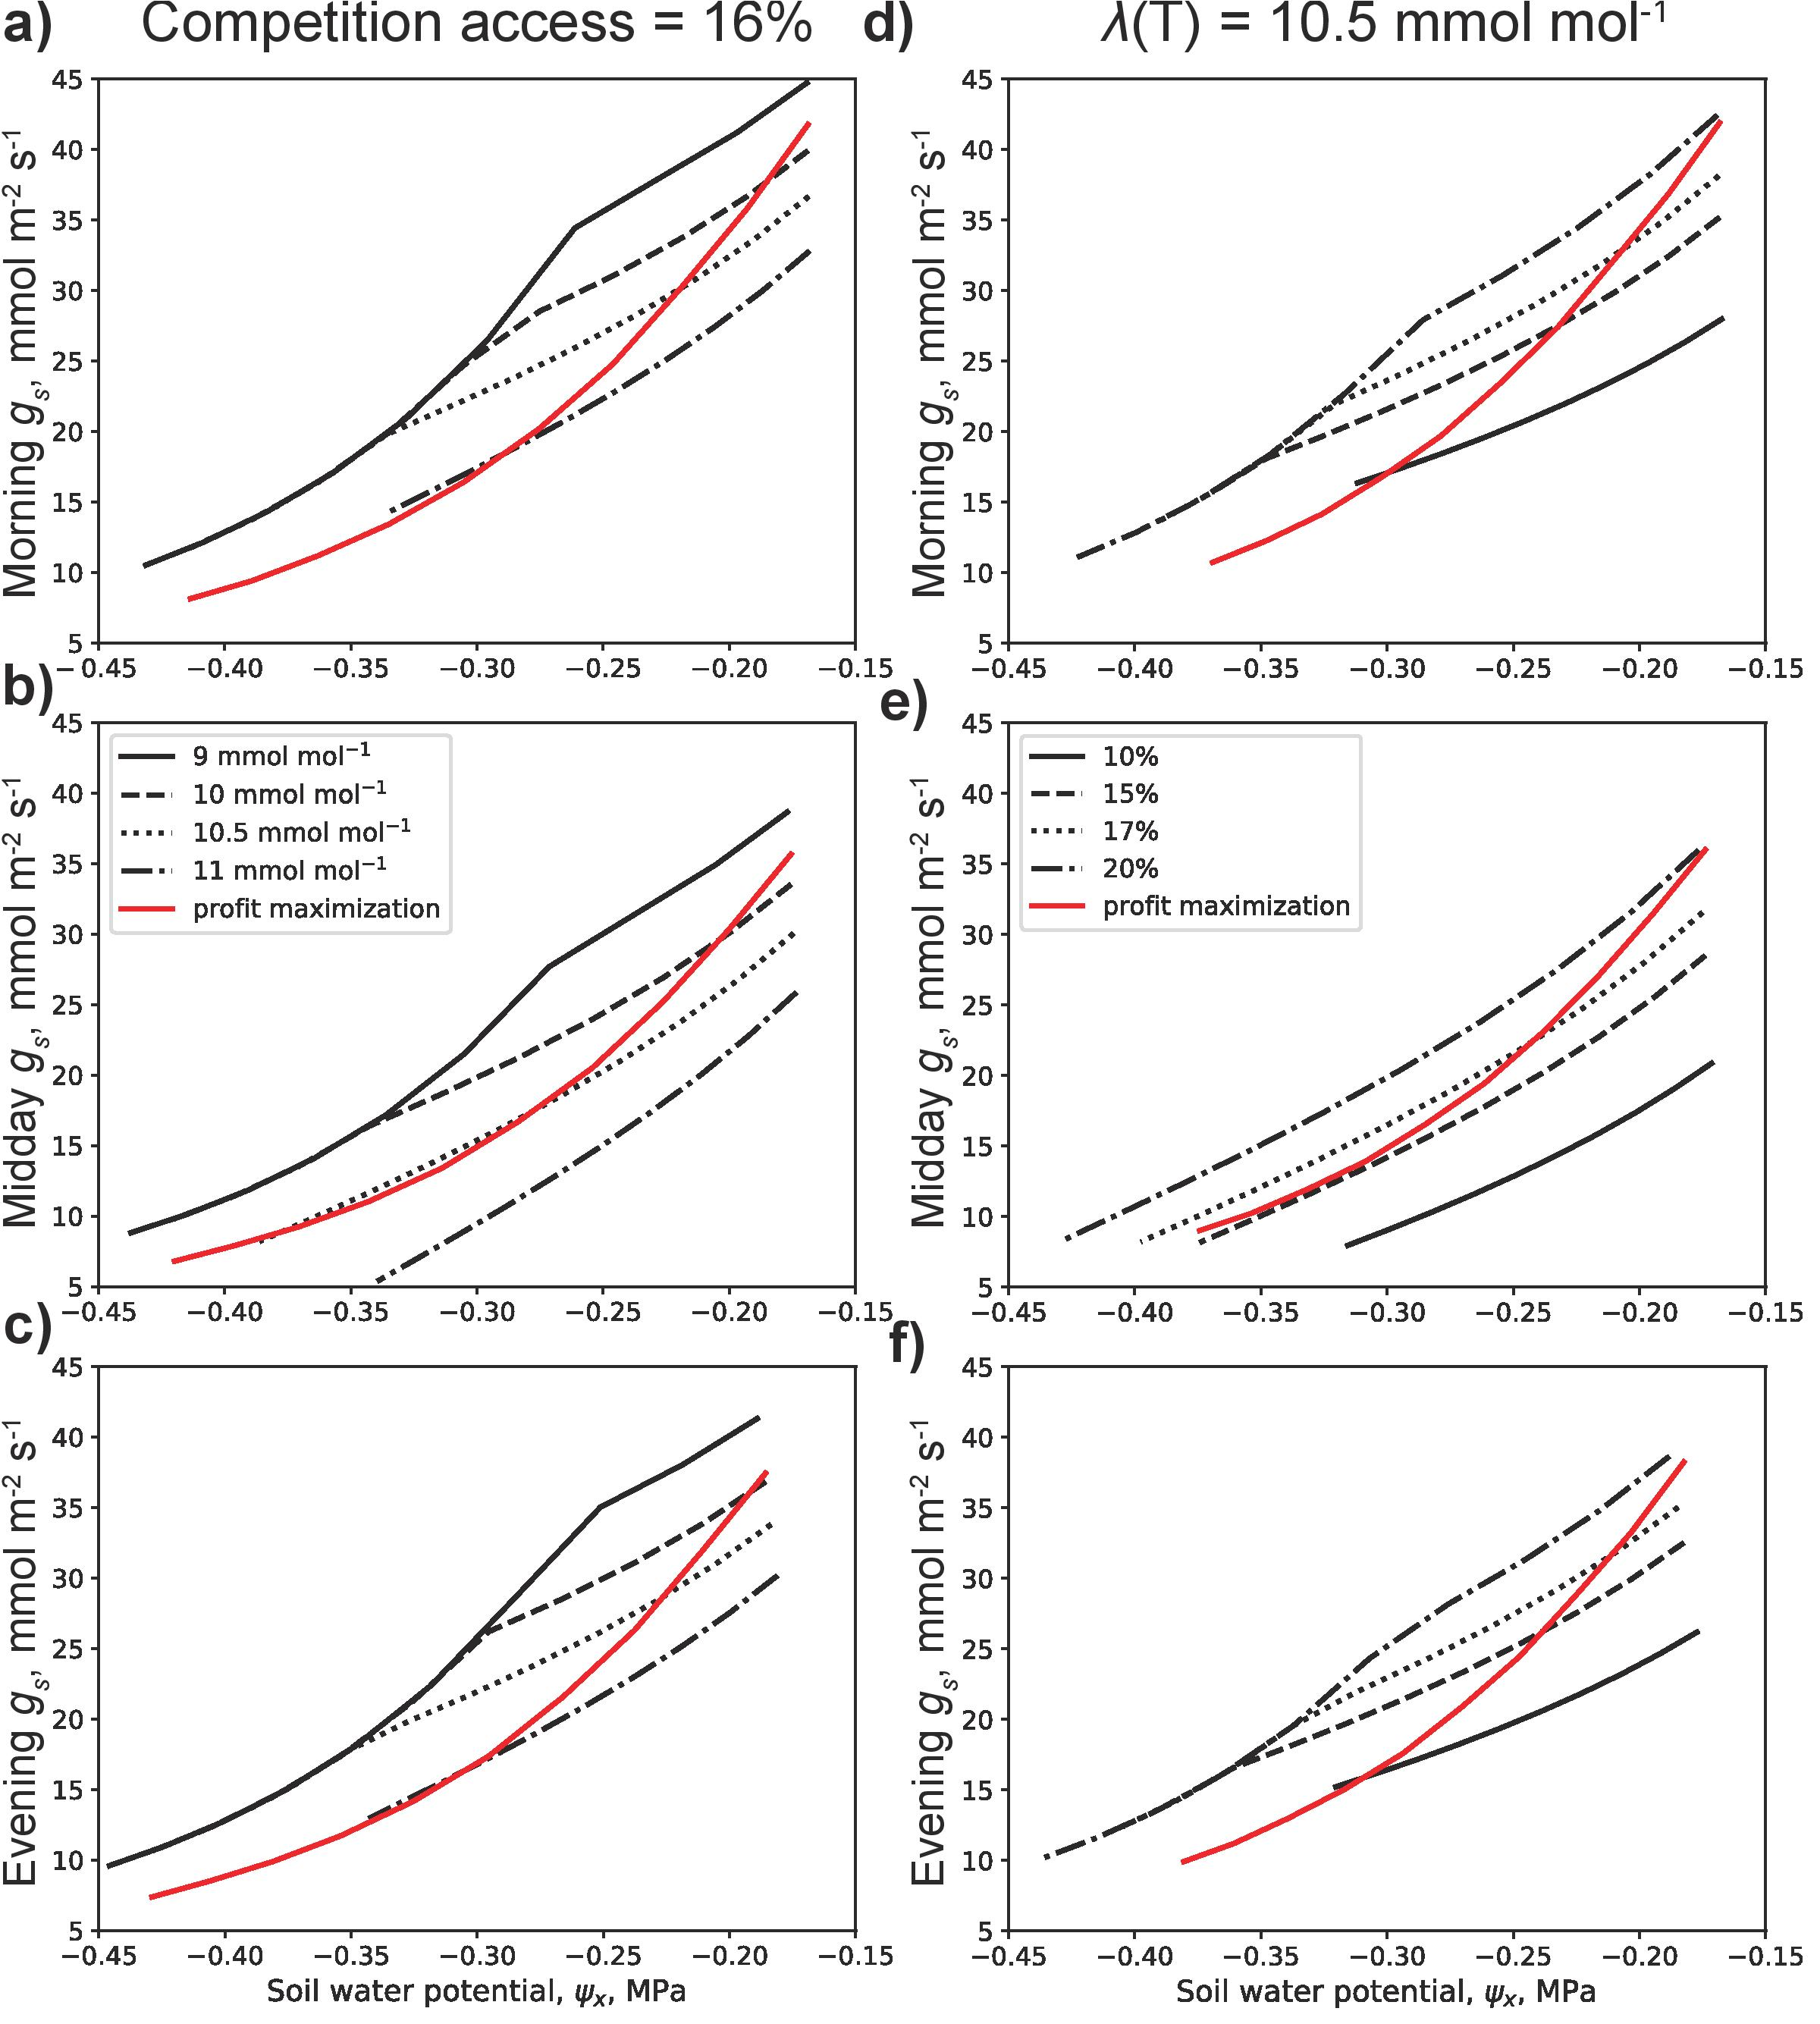
\includegraphics[scale=0.75]{profit_compare.jpg}   
    \end{center}
    \caption{Comparison between the dynamic optimality principle with plant hydraulic constraints and the profit maximization technique. In all panels, the plant is modeled with vulnerability curve (VC) parameters $\psi_{63} = -1.5$ MPa, $s=4$, and $g_{rl,max} = 2$ mmol m$^{-2}$ MPa$^{-1}$ s$^{-1}$. The plant competes with plants of similar VC and behavior who have access to a certain percentage of the modeled plant's rooting zone water. This percentage is called the competition access percentage. Panels a,b, and c vary the terminal marginal water use efficiency $\lambda(T)$ at the end of drydown $t=T$ while keeping the competition access constant at 16\%. Panels a,b, and c like panels d,e, and f show the sensitivity of morning, midday, and evening  stomatal conductance $g_s$ to soil water potential $\psi_x$, respectively. Panels d,e, and f keep $\lambda(T) = 10.5$ mmol mol$^{-1}$ while varying the competition access.} 
    \label{fig:profit_compare}
\end{figure}


\clearpage

%%Figures, tables, and images will be published under a Creative Commons CC-BY licence and permission must be obtained for use of copyrighted material from other sources (including re-published/adapted/modified/partial figures and images from the internet). It is the responsibility of the authors to acquire the licenses, to follow any citation instructions requested by third-party rights holders, and cover any supplementary charges.

\subsection{Tables}
% Tables should be inserted at the end of the manuscript. Please build your table directly in LaTeX.Tables provided as jpeg/tiff files will not be accepted. Please note that very large tables (covering several pages) cannot be included in the final PDF for reasons of space. These tables will be published as \href{http://home.frontiersin.org/about/author-guidelines#SupplementaryMaterial}{Supplementary Material} on the online article page at the time of acceptance. The author will be notified during the typesetting of the final article if this is the case. 


\begin{table}[h]
    \centering
    \begin{tabular}{l l l l}
        Symbol & Description & Value & Unit \\
        \hline
        \multicolumn{4}{l}{}\\
        \multicolumn{4}{l}{\textit{Soil and root hydraulic properties}}\\
        \hline
        % \multicolumn{4}{l}{}\\
        $\psi_{sat}$ & Saturation water potential & -1.5 & kPa\\
        $\psi_x$ & Soil water potential & & MPa\\
        $x$ & relative soil moisture & & m$^{3}$ m$^{-3}$\\
        $g_{sr,max}$ & Maximum ground area specific soil-root conductance & $0.72 * 10^{-3}$ & kg s m$^{-3}$ \\
        $g_{sr}$ & Ground area specific soil-root conductance & & kg s m$^{-3}$\\
        $b$ & Power law dependence parameter with $\psi_x$ & 3.1 & \\
        RAI & Root area index & 10 & m$^{2}$ m$^{-2}$\\
        $d_r$ & Average fine root diameter & 1 & mm \\
        $Z_r$ & Effective rooting depth & 0.3 & m\\ 
        $U$ & Uncontrolled losses of soil water & & mmol m$^{-2}$ s$^{-1}$\\
        \hline
        \multicolumn{4}{l}{}\\
        \multicolumn{4}{l}{\textit{Above-ground plant hydraulic properties}}\\
        \hline
        $g_{rl,max}$ & Maximum leaf area specific root-leaf conductance & 2 & mmol m$^{-2}$ s$^{-1}$ MPa$^{-1}$ \\
        $g_{rl}$ & Leaf area specific root-leaf conductance & see figure \ref{fig:grl} & mmol m$^{-2}$ s$^{-1}$ MPa$^{-1}$ \\
        $\psi_{63}$ & water potential at which $g_{rl} \approx 0.37 g_{rl,max}$ & see figure \ref{fig:grl} & MPa \\
        $s$ & Shape parameter of the vulnerability curve & see figure \ref{fig:grl} &  \\
        $g_s$ & Leaf area specific stomatal conductance & see figures \ref{fig:WUS_no_comp}, \ref{fig:WUS_comp} & mmol m$^{-2}$ s$^{-1}$ \\
        LAI & Leaf area index & 1.5 & m$^{2}$ m$^{-2}$\\
        \hline
        \multicolumn{4}{l}{}\\
        \multicolumn{4}{l}{\textit{Environmental properties}}\\
        \hline
        VPD & Vapor Pressure Deficit & see figure \ref{fig:environment} & mmol mol$^{-1}$\\
        $T_a$ & Atmospheric temperature & see figure \ref{fig:environment} & K \\
        PAR & Incoming photosynthetically active radiation & see figure \ref{fig:environment} & $\mu$mol m$^{-2}$ s$^{-1}$ \\
        \hline
        \multicolumn{4}{l}{}\\
        \multicolumn{4}{l}{\textit{Optimization results}}\\
        \hline
        $E(t)$ & Leaf area specific transpiration rate & & mmol m$^{-2}$ s$^{-1}$\\
        $A(t)$ & Leaf area specific carbon assimilation rate & & mmol m$^{-2}$ s$^{-1}$\\
        $\lambda (t)$ & Lagrange multiplier of the soil water balance constraint & & mmol mol$^{-1}$\\
        $L(t)$ & Augmented lagrangian & & mmol m$^{-2}$ s$^{-1}$\\
        $J$ & Objective function to be maximized & & mmol m$^{-2}$\\
        $T$ & Drydown period & 10 & days\\
        $J_T$ & Terminal gain term & & mol nol$^{-1}$\\
    \end{tabular}
    \caption{Symbols of soil, plant, and environmental properties along with their description, values, and units. These values correspond to the Blodgett forest data mentioned in subsection 2.8. Values for specific simulations will be mentioned in the simulation description and in the corresponding figure caption.}
    \label{tab:props}
\end{table}


% \section{Nomenclature}

% \subsection{Resource Identification Initiative}
% To take part in the Resource Identification Initiative, please use the corresponding catalog number and RRID in your current manuscript. For more information about the project and for steps on how to search for an RRID, please click \href{http://www.frontiersin.org/files/pdf/letter_to_author.pdf}{here}.

% \subsection{Life Science Identifiers}
% Life Science Identifiers (LSIDs) for ZOOBANK registered names or nomenclatural acts should be listed in the manuscript before the keywords. For more information on LSIDs please see \href{http://www.frontiersin.org/about/AuthorGuidelines#InclusionofZoologicalNomenclature}{Inclusion of Zoological Nomenclature} section of the guidelines.


% \section{Additional Requirements}

% For additional requirements for specific article types and further information please refer to \href{http://www.frontiersin.org/about/AuthorGuidelines#AdditionalRequirements}{Author Guidelines}.

\section*{Conflict of Interest Statement}
%All financial, commercial or other relationships that might be perceived by the academic community as representing a potential conflict of interest must be disclosed. If no such relationship exists, authors will be asked to confirm the following statement: 

The authors declare that the research was conducted in the absence of any commercial or financial relationships that could be construed as a potential conflict of interest.

\section*{Author Contributions}

AM and YL contributed to the modelling effort. AM, GK, and SS designed the direction of this work. All authors contributed to the analysis of the results and in drafting the manuscript.

\section*{Funding}
G. Katul, A. Mrad, M. Nakad, and J.C. Domec acknowledge support from the U.S. National Science Foundation (NSF-EAR-1344703,NSF-AGS-1644382, and NSF-IOS-1754893).

\section*{Acknowledgments}
This work used eddy covariance data acquired and shared by the FLUXNET community, including these networks: AmeriFlux, AfriFlux, AsiaFlux, CarboAfrica, CarboEuropeIP, CarboItaly, CarboMont, ChinaFlux, Fluxnet-Canada, GreenGrass, ICOS, KoFlux, LBA, NECC, OzFlux-TERN, TCOS-Siberia, and USCCC. The ERA-Interim reanalysis data are provided by ECMWF and processed by LSCE. The FLUXNET eddy covariance data processing and harmonization was carried out by the European Fluxes Database Cluster, AmeriFlux Management Project, and Fluxdata project of FLUXNET, with the support of CDIAC and ICOS Ecosystem Thematic Center, and the OzFlux, ChinaFlux and AsiaFlux offices.


\section*{Appendix 1: Deriving the soil-root-atmosphere conductance}

The soil-root-atmosphere conductance include both the conductances of soil to root and root to leaf in series. It is defined as the marginal increase in transpiration rate $E$ with an increase in leaf water potential $\psi_l$ \citep{sperry_what_2015}. One can write:
\begin{equation}
    \label{eqn:g_sl}
    g_{sl} = \frac{\partial E}{\partial \psi_l},
\end{equation}
where $g_{sl}$ is the soil to leaf water conductance. Because of mass conservation, $E$ is equal to water flow from soil to root ($E_{sr}$) and from root to leaf ($E_{rl}$) (equation \ref{eqn: mass_cons}).
Taking the derivative of $E_{sr}$ with respect to $\psi_l$:
\begin{equation}
    \label{eqn:Esr_psil}
    g_{sl} (\psi_l) = - g_{sr} (\psi_x) \frac{\partial \psi_r}{\partial \psi_l} (\psi_l).
\end{equation}
Taking the derivative of $E_{rl}$ with respect to $\psi_l$:
\begin{equation}
    \label{eqn:Erl_psil}
    g_{sl} (\psi_l) = g_{rl} (\psi_r) \frac{\partial \psi_r}{\partial \psi_l} (\psi_l) - g_{rl} (\psi_l).
\end{equation}
Equating $g_{sl}$ from both equations \ref{eqn:Esr_psil}, \ref{eqn:Erl_psil}:
\begin{equation}
    \label{eqn:psir_psil}
    \frac{\partial \psi_r}{\partial \psi_l} (\psi_l) = \frac{g_{rl} (\psi_l)}{g_{rl} (\psi_r) + g_{rl} (\psi_r)}.
\end{equation}
One now obtains a closed form relation for $g_{sl}$:
\begin{equation}
    \label{eqn:gsl_complete}
    g_{sl} (\psi_l) = \frac{g_{rl} (\psi_l) g_{sr} (\psi_x)}{g_{rl} (\psi_r) + g_{sr} (\psi_x)}.
\end{equation}
One can also find the maximum possible soil to leaf conductance at different soil moisture values by replacing all water potential in equation \ref{eqn:gsl_complete} with $\psi_x$ as follows:
\begin{equation}
    \label{eqn:gsl_max}
    g_{sl,max} = \frac{g_{rl} (\psi_x) g_{sr} (\psi_x)}{g_{rl} (\psi_x) + g_{sr} (\psi_x)}.
\end{equation}
Now, the critical leaf water potential $\psi_{l,crit}$ is found by equating $g_{sl}(\psi_l) = 0.05 g_{sl,max}$ from equations \ref{eqn:gsl_complete}, \ref{eqn:gsl_max}.



\section*{Appendix 2: the effect of competitive plant transpiration on $\lambda$}
Equation \ref{eqn:simulation_co_state} expresses $d \lambda / dt$ as a function of $\partial E_{comp} / \partial x$ where $E_{comp}$ is the competitive plant's water use from the modeled plant's rooting zone water. As explained in the paragraph following equation \ref{eqn:uncontrolled_losses}, $E_{comp}=0.2E$ based on the assumption that both modeled plant and competitive plant have the same VC and have the same rooting zone water content. Therefore, we can write:
\begin{equation}
    \label{eqn:E_comp}
    E_{comp} = g_{sr,comp}(\psi_x)(\psi_x - \psi_{r,comp}),
\end{equation}
where $\psi_x$ corresponds to the water potential in the vicinity of the modeled plant's rooting zone and $\psi_{r,comp}$ is the effective root water potential of the competitive plant. $g_{sr,comp} = 0.2 g_{sr}$ because competitive RAI is less than modeled plant RAI in the rooting zone of interest (equation \ref{eqn:soil_root}) such that the competitive plant only has access to 20\% of the modeled plant's rooting zone water (equations \ref{eqn:simulation_co_state}, \ref{eqn:uncontrolled_losses}). Since $\psi_{r,comp}$ responds to the competitive plant's rooting zone water content and not on the model plant's, we write $\partial \psi_{r,comp} / \partial x = 0$ because $x$ is the modeled plant's rooting zone water content. Therefore:
\begin{equation}
    \label{eqn:Ecomp_x}
    \frac{\partial E_{comp}}{\partial x} = 0.2 \frac{\partial \psi_x}{\partial x} \Bigg[ \frac{\partial g_{sr}}{\partial \psi_x} (\psi_x - \psi_{r,comp}) + g_{sr}(\psi_x) \Bigg].
\end{equation}

Note how the result of equation \ref{eqn:Ecomp_x} is different from $\partial E / \partial x = 0$ where $E$ is the modeled plant's transpiration rate.

% Please see the availability of data guidelines for more information, at https://www.frontiersin.org/about/author-guidelines#AvailabilityofData

\bibliographystyle{frontiersinSCNS_ENG_HUMS} % for Science, Engineering and Humanities and Social Sciences articles, for Humanities and Social Sciences articles please include page numbers in the in-text citations
%\bibliographystyle{frontiersinHLTH&FPHY} % for Health, Physics and Mathematics articles
\bibliography{references}

%%% Make sure to upload the bib file along with the tex file and PDF
%%% Please see the test.bib file for some examples of references

% \section*{Figure captions}

% %%% Please be aware that for original research articles we only permit a combined number of 15 figures and tables, one figure with multiple subfigures will count as only one figure.
% %%% Use this if adding the figures directly in the mansucript, if so, please remember to also upload the files when submitting your article
% %%% There is no need for adding the file termination, as long as you indicate where the file is saved. In the examples below the files (logo1.eps and logos.eps) are in the Frontiers LaTeX folder
% %%% If using *.tif files convert them to .jpg or .png
% %%%  NB logo1.eps is required in the path in order to correctly compile front page header %%%

% \begin{figure}[h!]
% \begin{center}
% 
\includegraphics[width=10cm]{logo1}% This is a *.eps file
% \end{center}
% \caption{ Enter the caption for your figure here.  Repeat as  necessary for each of your figures}\label{fig:1}
% \end{figure}


% \begin{figure}[h!]
% \begin{center}
% \includegraphics[width=15cm]{logos}
% \end{center}
% \caption{This is a figure with sub figures, \textbf{(A)} is one logo, \textbf{(B)} is a different logo.}\label{fig:2}
% \end{figure}

%%% If you are submitting a figure with subfigures please combine these into one image file with part labels integrated.
%%% If you don't add the figures in the LaTeX files, please upload them when submitting the article.
%%% Frontiers will add the figures at the end of the provisional pdf automatically
%%% The use of LaTeX coding to draw Diagrams/Figures/Structures should be avoided. They should be external callouts including graphics.

\end{document}
